\documentclass[12pt,a4paper]{report}
\oddsidemargin 0.25in
\evensidemargin 0.25in
\textwidth 6in
\linespread{1.5}
\topmargin 0.5in
\usepackage{enumerate}
\usepackage[lined,linesnumbered,ruled]{algorithm2e}
\usepackage{tabularx}
\usepackage{amsmath, amsthm, bbm, amsfonts, fancybox, times, amssymb, array, graphicx, hyperref, mathrsfs, cite}
\usepackage{bm}
\usepackage{fancyheadings}
\usepackage{appendix}
\usepackage{booktabs}
\usepackage{epsfig}
\usepackage{subfigure}
\usepackage{algorithmic}
\usepackage{balance}
\setcounter{secnumdepth}{3}
\newtheorem{Def}{Definition}
\newtheorem{theorem}{Theorem}
\graphicspath{{figs/}}

%----------------------------------------------------------------------------------------------------------------

\begin{document}
\pagestyle{empty}
\begin{center}
\LARGE \textbf{Compressed Sensing for Wideband Signal Processing}
\end{center}
\vspace{1cm}

\begin{figure}[!h]
  \begin{center}
    
\includegraphics[width=4.5cm]{ntu_logo.eps}
  \end{center}
\end{figure}

\vspace{0.5cm} \large
\begin{center}
\textbf{Chen Hao}
\end{center}
\vspace{0.3cm}

\begin{center}
\textbf{School of Computer Engineering}
\end{center}
\vspace{0.5cm} \normalsize

\begin{center}
A Process report submitted to the School of Computer Engineering \\
of Nanyang Technological University\\
\vspace{0.2cm}
in partial fulfillment of the requirements for the\\
degree of Doctor of Philosophy \\
\vspace{0.6cm} Supervisor: Assoc. Prof. Vun Chan Hua\\
\vspace{0.6cm}

January 2015
\end{center}
\normalsize
\newpage
\mbox{}
\newpage
%-----------------------------------------------------------------------------------------------------------------
\newpage
\Large
\begin{abstract}
\normalsize

\indent Signal processing have been widely deployed in many computational applications in areas such as image processing, video conferencing, smart sensors network, and other real-time processing technologies. Many signal processing systems also involve signal sampling and conversion, where one of the most crucial limitations lies in the sampling theory (the Nyquist sampling rate or Shannon theory, which states the minimum two time sampling rate requirement.) Due to limited data processing and storing capability found in many wireless communication systems, excessive data samples will negatively affect their performance and power efficiency, and hence forms the bottleneck of entire digital systems. 

As a novel paradigm for signal processing and acquisition, the compressive sensing or compressed sensing (CS) technique, is identified to have great potential for resolving the problems mentioned above. The CS theory has been proven to be suitable for numerous computer science and electronic engineering based applications, where it is possible to overcome the limitation of the traditional sampling theory. 

The main idea of the research work is to further extend the CS based techniques to wireless systems. Using this approach, the novel systems will be proposed that encompass various areas such as data compression, data acquisition, data storage, data transmission, optimal recovery and processing. Specifically, we stress the focus on the wideband signal processing since the requirement of sampling wideband spectrum generates comparatively higher pressure than narrow band signal processing, hence dealing with wideband acquisition and processing is full of importance and necessary. 

Following this idea, in this report, we focus our research aims to the areas involving extremely high frequency acquisition and processing scenarios -- the ultra wideband (UWB) positioning and cognitive spectrum sensing (CSS). For many ultra wideband (UWB) communication systems, how to receive the signal over GHz at lower cost is a crucial problem. For cognitive radios (CR), how to efficiently sense the occupation of active primary users (PU) while not creating interference to PUs is still an important and open issue.

In order to solve these problems, this report studies novel approaches which respectively embed the CS framework into those systems. In our proposed CS-UWB system, random projection is located at transmitters to support CS framework while sub-Nyquist low-rate ADCs are implemented at receivers. As a result, not only the accuracy is improved but also the sampling cost is significantly reduced. On the other hand, we study the recent CS-CSS systems' performance and analyize the cost of embedding CS into such systems. The analysis result indicates us that rather than fully reconstructing the CS measurements, the partial recovery or extraction useful information directly from unrecovered signals is more attractive and suitable in many cognitive radio spectrum sensing cases since it improves the real-time capability while keeps low sampling rate in CS. This idea intrigues our future research directions and motivations aiming at compressive signal processing (CSP, including compressive measurements analysis and partial support recovery etc) for wideband signal processing in cognitive radios and ultra wideband systems.

The organization this report is presented as: Chapter \ref{C:compressed_sensing} firstly presents the overview of compressed sensing theory and its applications, and then focuses on wideband signal acquisition hardware design which relates to our survey for recent CS-ADC architectures. Then the following chapter \ref{C:compressive_uwb_positioning} presents our related work in compressive UWB positioning systems. What's more, the chapter \ref{C:wideband_css} introduces the compressive spectrum sensing for cognitive radios, but points out the limitation due to CS fully reconstruction. Finally, the chapter \ref{C:csp_css} proposes our recommenced future research on compressive signal processing based cognitive spectrum sensing.
\end{abstract}

\newpage
\begin{center}
\Large
\vspace{3cm} \textbf{Acknowledgements}
\end{center}
\normalsize
\indent \indent I would like to express my sincere and great gratitude to my supervisor, Assoc Prof. Vun Chan Hua for his kind guidance and encouragement. It is a great honor to work with him. I own my sincere appreciate to all my friends in CeMNet. Without their help, my first year study and research in NTU can not process well.


\newpage
\makeatletter
\let \asas \ps@plain
\let \ps@plain \ps@empty
\makeatother \large
\tableofcontents
\listoffigures
\listoftables

\newpage
\addtolength{\headheight}{3pt} \pagestyle{fancy}
\setlength{\headrulewidth}{0.1pt}
\renewcommand{\chaptermark}[1]{\markboth{\chaptername\ \thechapter. #1}{}}
\lhead{\fancyplain{}{\bfseries\footnotesize\sc\leftmark}} \rhead{}
\addtolength{\headsep}{-0.1in}
\cfoot{\fancyplain{}{\bfseries\rm\thepage}}
\pagenumbering {arabic}     % Use arabic number for the page number of main body
\normalsize
%-------------------------------------------------------------------------------------------------------------

\chapter{Introduction}\label{C:Introduction}
%%require: strong-motiv, clear-focus, induce-logic
%%require: fig, data, trends
%%require: cs-wireless-intro, general apps.
%%require: good history

\indent \indent This chapter firstly introduces the challenges in signal processing with respect of signal acquiring limitation due to Nyquist sampling theorem, and then turn to focus on the compressed sensing (CS) for solving the problem. Next, potential CS based wireless applications, especially those for wideband signal processing, are proposed. Besides, it is still important to point out that there still exist several gaps between CS theory and its hardware implementations involving constraints like energy-cost, non-ideal model mismatch, real-time capacity. These gaps motivate our investigations and future research. At last, the organisation of the entire report is presented.

\section{Challenges of Signal Processing}
\indent \indent Signal processing is to processes or transfers information that contained in real world signals. The principle of signal processing is firstly founded by Alan V. Oppenheim and Ronald W. Schafer, and so far widely developed and related to modelling, analysis, extraction, learning, security etc \cite{moura2009signal}. 

Once Oppenheim and Schafer stated that the "digitisation" can be applied in signal processing \cite{oppenheim1989discrete}, signal processing is tightly linked with digitisation, for it can provide additional benefits such as compression and error detection \cite{broesch2008digital}. Consequently, the digital signal processing (DSP) algorithms and devices have been widely deployed in image processing, video conferencing, smart sensors network, and other real-time processing tasks. Its applications are also increasingly implemented in the form of embedded systems such as mobile and wireless devices\cite{mamaghanian2011compressed}, aerospace equipment, and biomedical instruments\cite{lustig2008compressed}.

However, during the digitisation, signal acquiring and quantification are always highly restricted by the sampling rate, because the famous Shannon theory states that the minimum sampling rate should be at least twice as the most highest frequency components of original signals (we also call it the Nyquist rate). As a result, DSP devices have to match the high sampling rate requirements in their input front-end. What's worse, because the input front-end of DSP is the first stage of the entire system, the limitation of sampling rate correspondingly influences the further stages for data processing and storage.

Therefore, the limitation in signal sampling not only increases the design complexity to analog-to-digital converters (ADCs), which is the input front-end of DSP, but increases the data size of storage, as well as the scale for further data processing. Consequently, the power consumption, computational cost, and commercial design cost become raising. What's worse, as the trend of developing DSPs requires faster sampling, larger dynamic range, higher dimensional data, low-energy consumption and high sensing mobility \cite{danckaert1999strategy}, if we cannot solve the sampling limitation, then not only sampling itself, which relates to faster sampling, larger range and sensing mobility, but also burden storage for high dimensional data and energy saving for low-energy consumption, will be significantly affected. In one word, all requirement refers to the key problem of sampling. From this aspect, solving the limitation in signal sampling is by no means tolerable for modern signal processing devices.

\section{Compressed Sensing Overview}
\indent \indent Fortunately, the compressed sensing (CS) presents us an useful approach to extract sparse interests of signal BELOW the Nyquist rate. The CS framework provides high possibility to reconstruct original signals through few randomly sampled data than traditional Nyquist sampling method. Using the l1-norm minimisation, figure \ref{I:intro-cs} demonstrates the recovery results between CS reconstruction and conventional recovery. From the comparison, we can conclude that the CS successfully recover the sparse spectrum information from the original signals. The following paragraphs presents related topics for CS. 

\begin{figure}
\label{I:intro-cs}
\centering
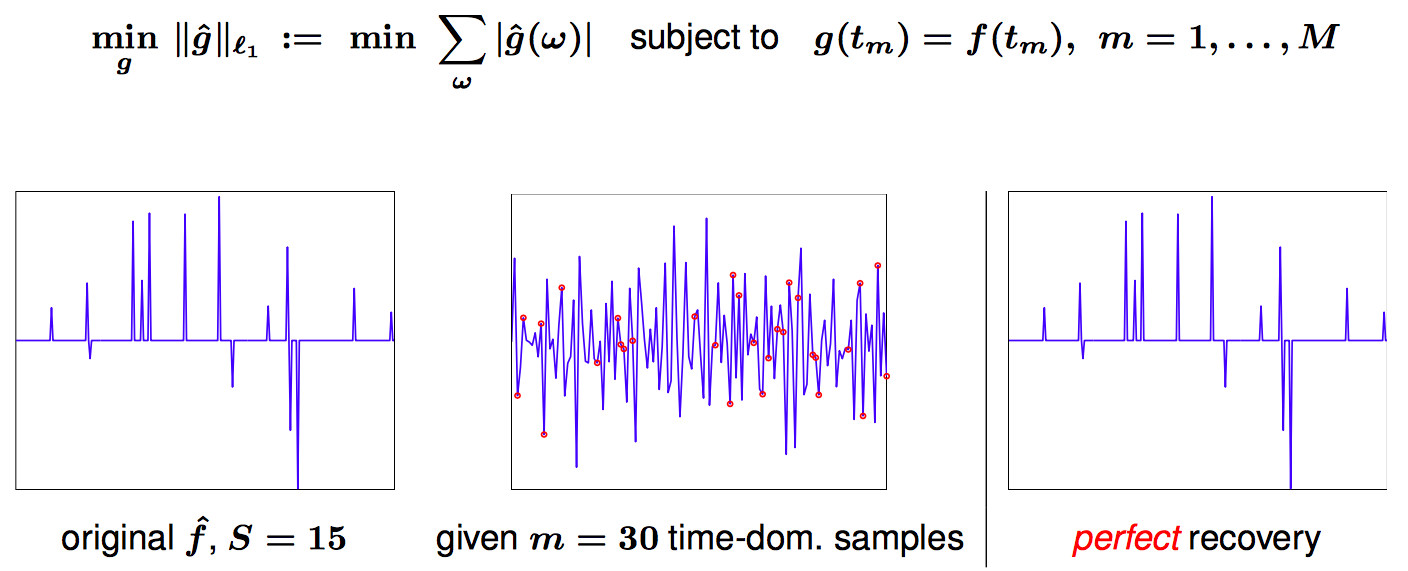
\includegraphics[width=5.0in]{figs/cs-reconst-intro.png}
\DeclareGraphicsExtensions.
\end{figure}

\paragraph{Sparsity}
The goal of signal processing is to reconstruct the original signal from a stream of samples. In the procedure of reconstruction, fewer samples of information is needed if the prior knowledge of signal’s frequencies is clear. By appropriate representation, e.g. Fourier basis representation, natural signals are always represented by few significant coefficients, and termed as sparse information. Mathematically, the sparse information can be presented if assuming the signal of $x \in R^N$ can be decomposed by a group of basis $\Psi$, where $k << N$:  
\begin{equation}
x=\Psi s=\sum_{l=1}^{K}\psi_l s_l  
\end{equation}
Here $x$ is a linear combination of $K$ basis chosen from $\Psi$, and $s$ is the corresponding coefficients of representing $x$ in the domain constructed by the basis $\Psi$. 

\paragraph{Incoherence}
The incoherence presents the idea that signals $x$ containing a sparse representation in basis $\Psi$ must be spread out in the basis domain in which they are acquired \cite{candes2008introduction}. For instance, the spike is spread out in the frequency domain. In other words, the incoherence indicates the sampling/sensing waveforms have an extremely dense representation in the basis. 

\paragraph{Relevance}
Similarly, the wavelets compression \cite{chui1992introduction} e.g JPEG2000 also develops the sparse information in natural images. It represents images into approximately sparse and ignores large amount of small (nearly zero) coefficients. This is the reason why the wavelets only remain small size data while keeping the image with high information. For instance, using wavelets, natural images can be compressed into a relative small size ( < 5 percent of original size) while still keeping high quality. An example is demonstrated in figure \ref{I:wavelet-intro}.

\begin{figure}
\label{I:wavelet-intro}
\centering
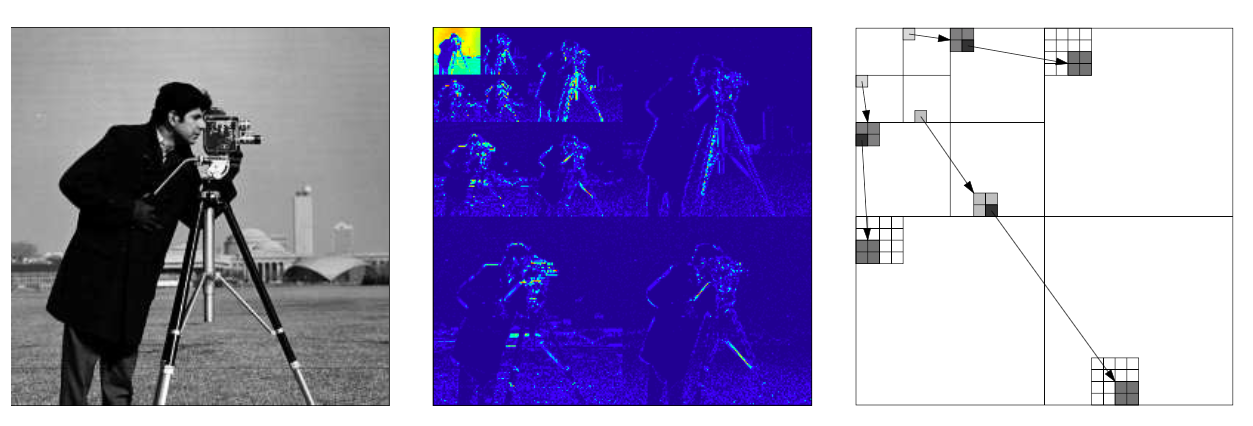
\includegraphics[width=5.0in]{figs/wavelets-intro.png}
\DeclareGraphicsExtensions.
\caption{An example of Haar-wavelet decomposition. Only light coefficients are significant. Dark ones are nearly zero and can be neglected.}
\end{figure}

According to the principles of wavelets, the steps of this approach can be described as sample then compress. However, in the step of sampling, the Nyquist rate is still required. This is the main difficult between CS and wavelets, since the CS can overcome the limitation provided by the Nyquist rate. 

\paragraph{Develop of CS}
Around 2005, Terence Tao, David Donoho, Emmanuel Candès mathematically proved that using random selection, the low-rate sampled measurements can reconstruct original data with high possibility, using $l1$-norm minimisation \cite{candes2006robust,baraniuk2007compressive} shown as equation \ref{eq_l1_min}. 
\begin{equation}
\label{eq_l1_min}
\hat s = \arg\min \| s \|_1 \quad s.t. \quad  y = A s
\end{equation} 
, where it has been proven that only $O(K\ln(N/K))$ samples are needed if matrix $A$ are incoherent with $s$. One of the best choice for the independence is to use i.i.d variables (independent and identically distributed variables) constructed matrix such as the Gaussian matrix. Further, more constructed matrix like Bernoulli matrix, partial Fourier matrix are proven suitable for CS. Therefore, CS provides a novel random sampling paradigm which is applicable for modern signal sampling and data processing with low rate. 

\section{Typical Compressed Sensing Applications}

\paragraph{Compressive Radar Systems}
Compressed sensing has showed outstanding feature in  in reducing the sampling rate in many wireless applications, e.g. radar systems, since many wireless devices communicate at high frequency which lead to heavy burden in sampling task so that the CS can be used to reduce the sampling rate at receivers \cite{bajwa2006compressive}. In addition, in radar systems, it's necessary to have capacity to acquire wideband signals with different signal templates, such as TV bands, satellite signals, cell-phone informations etc. Traditional method always require filter-banks to down-sample these signals, while the CS can help original system directly sense the various of wide-band signal, or with less filters. The figure \ref{I:cs-radar-intro} presents a wide-band signal monitoring and processing radar system that receives signals from a variety of sources.

\begin{figure}
\label{I:cs-radar-intro}
\centering
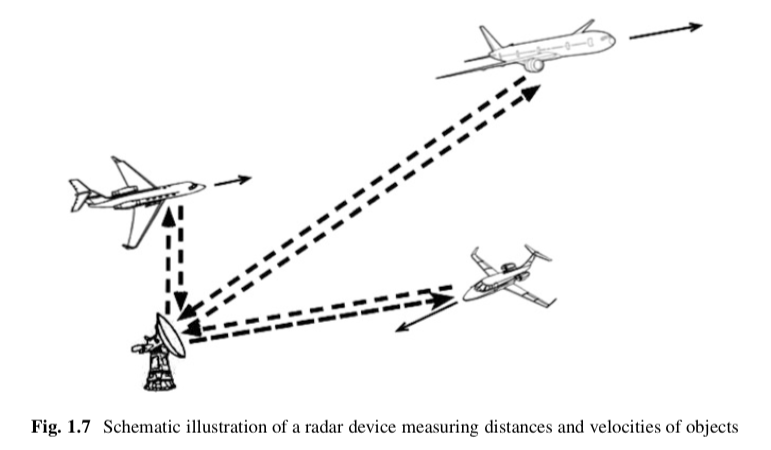
\includegraphics[width=5.0in]{figs/cs-radar-intro.png}
\DeclareGraphicsExtensions.
\end{figure}

\paragraph{Compressive Single Pixel Camera}
Different from the wavelets, compressed sensing requires little samples which reduce the energy during image acquisition. For instance, the CS framework is implemented for single-pixel cameras by  Rice University \cite{baraniuk2008single}. This new CS-camera directly acquires random projected samples from a image without first gain the pixels, and the random projected samples are collected by digital micro-mirror array, which optically reflects a linear projection of the image onto pseudo-random binary patterns.

\begin{figure}
\centering
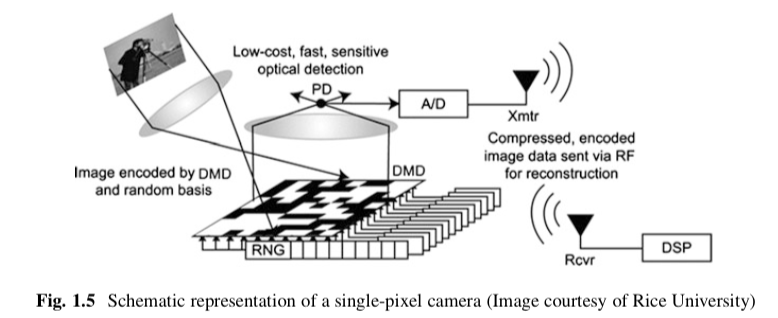
\includegraphics[width=5.0in]{figs/cs-camera-intro.png}
\DeclareGraphicsExtensions.
\end{figure}

\paragraph{Magnetic Resonance Imaging}
Magnetic resonance imaging (MRI) is a widely used technology in medical imaging, applications such as brain scanning, angiography, and dynamic heart imaging are necessary for medical diagnosis \cite{foucart2013mathematical}. However, this imaging tool burdened by an inherently slow data acquisition process since traditional approaches based on the Shannon sampling theorem requires long-time scanning if the high-resolution images are required \cite{lustig2007sparse}. In the cases that the patients cannot be expected to hold statically for long-period (e.g. children are too impatient to sit for more than minutes). The embedding CS to MRI has the potential to significantly reduce the scan time. 

\begin{figure}
\label{I:cs-mri-intro}
\centering
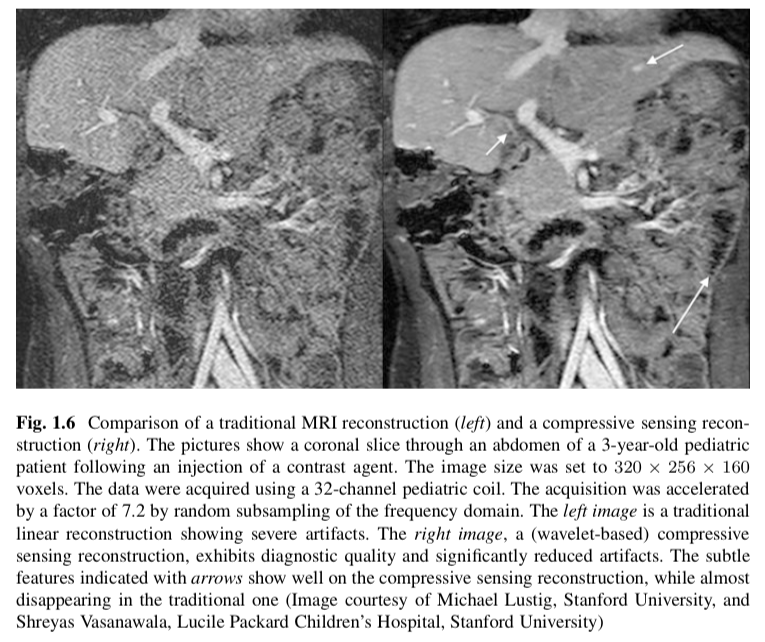
\includegraphics[width=5.0in]{figs/cs-mri-intro.png}
\DeclareGraphicsExtensions.
\caption{The comparison of a traditional MRI reconstruction (left) and a compressive sensing reconstruction (right).}
\end{figure}

\section{Compressive Wireless Communication}
\indent	\indent Over the past few decades, the demand for high frequency communication and wideband signal detection keeps increasing, which worsen the acquiring the situation. For instance, modern digital systems often require bigger data size, or higher rate communication (e.g. ultra-wideband), or more flexible networks (which emerges hybrid wireless devices, e.g. cognitive radio), and all the requirements highly rely on accurate and sensitive sampling approaches. Thus, enhancing the performance of sampling devices brooks no delay. 

Therefore, our study motivation derives from the problem of signal acquisition devices, especially for those who aims at collecting wideband / high frequency signals. An suitable research object is the wireless application, for many applications are communicating at high frequency, and becoming more and more depend on high performance receivers and detectors, as well as the novel sampling approaches. Fortunately, the compressed sensing (CS) presents us an useful approach to extract sparse interests of signal BELOW Nyquist rate. This novel approach motivates a large range of application in signal processing. The next section will introduce this method. 

In fact, although the CS framework solve the problem in Nyquist sampling rate theoretically, the gap between hardware applications and ideal cases still remain. For instance, as the CS theory often requires a true randomness in sampling approaches, while hardware implementations only provide pseudo-randomness instead. The constraints doesn't only stay in CS theory implementation, but design limitations or awareness such as energy consumption, real-time capability, design complexity etc. All the constraints bring about tradeoffs design schemes, so CS applications for wireless, signal processing is still an open issue. 

\subsection{Research Aims}
\indent \indent As an important application area for CS, wireless communication is always puzzled by high frequency transmission detection or wideband signal processing, e.g. radar systems. Those applications, to our best knowledge, are mainly focus on high frequency required scenarios, including multiple-input and multiple-output (MIMO), multiple access (MA), ultra-wideband (UWB), cognitive radio (CR).

In this report, we are more focusing on CS based wireless communication, especially aims at the physical layer and MAC layer. For research applications, we select two typical and popular applications, which  involves extremely high-frequency and wide bandwidth signal processing respectively -- the ultra-wideband  system and cognitive radio. 

\paragraph{Compressive Ultra-Wideband Positioning} 
The Ultra-Wideband (UWB) communication is widely used in wireless communication and associated with features as extreme wide transmission bandwidth, low-power consumption, shared spectrum resources in wide ranges etc. However, for many ultra wideband communication systems, how to energy-efficiently collect signals higher than GHz is a crucial problem. In order to solve these problems, we study the novel approach that embeds CS into the UWB positioning. In our proposed compressive UWB positioning system, random projection is located at transmitters to support CS framework while sub-Nyquist low-rate ADCs are implemented at receivers. As a result, not only the accuracy is improved but also the sampling cost is significantly reduced. The detailed design is introduced in chapter \ref{C:compressive_uwb_positioning}.

\paragraph{Compressive Cognitive Radio Spectrum Sensing}
Cognitive Radio (CR) has been attracting many attention due to its potential better utilisation for limited spectrum resources. However, for many cognitive radios, how to accurately and quickly sense the occupation of active primary users (PUs) without additional interference is a crucial problem. In order to solve this problems, we study the novel approach in chapter \ref{C:wideband_css} embedding CS into recent CR spectrum sensing techniques. Then we analyse the performance and cost for applying the CS. The analysis and discussion finally motivates us for future research on compressive signal processing (CSP) for cognitive spectrum sensing in chapter \ref{C:csp_css}.

\section{Problem Statement}\label{sct:problem_state}
\indent \indent In this chapter, we narrow the concerned problems to CS wireless hardware designs, mainly from two aspects: (1) Although the CS is outstanding for its significance in reducing the sampling rate, however, as a sacrifice, the reconstruction procedure is non-linear and full of complexity and difficulty. (2) Besides, CS sensing model hardware implementation is not easy and simple, for building absolute incoherent and independent sensing matrix is challenging (e.g. true randomness in Gaussian matrix can hardly be implemented in computer engineering field). The following problems open up some interesting issues for our research, and  some of them are focused in this report and some will be studied in our future works. 

\paragraph{Real-Time Capability}
The reconstruction algorithms for CS is non-linear, which indicates that the recovered data are not directly suitable for conventional digital signal processing where a simple linear recovery using cardinal sine interpolation is needed. Besides, some of the high accuracy reconstruction algorithms based on convex optimisation are time consuming, e.g. the basis pursuit's complexity is $O(N^3)$, which generates large time delay for further data processing, and do harm to the feed-back required devices. On the other hand, even though greedy method (e.g. the orthogonal matching pursuit's complexity is $O(kMN)$) has speed up the sunning time for CS reconstruction, the recovered data is located in different domain, e.g. original data is sampled in time domain while the recovered data in frequency or spatial domain. The domain mismatch sometimes require addition transforming task which generates more cost in time and energy. In one word, CS reconstruction make the real-time capability worse, and lead many CS techniques not suitable for feed-back required processing systems.  

\paragraph{Processing Flexibility}
Higher flexibility is one of the important trend and requirement for modern signal processing devices. In contrast to the task-specific hardware used in many classical acquisition systems, many hardware designed to use a compressive measurement protocol can be extremely flexible. 
A stylised future CS radar system demonstrate the potential signal processing pattern for wide-band signals:  In figure \ref{I:cs-radar-intro}, the CS radar receives various types of signals from televisions, cellphones, aeroplanes and satellites etc. However, the signals' templates are unknown to the system, such as signal-to-noise ratio and sparsity order which seriously affect the performance of detectors. Then what information should be collected ? How to accomplish matched filters ? Is adaptive selection needed ? These solutions sometimes computational expensive but not flexible enough. What's worse, the CS reconstruction is non-linear which does not match the traditional processing approaches and thus increase the analysis difficulty. 

\paragraph{Energy Efficiency}
Compressed sensing community has provided many hardware architectures for analog-to-digital information to build sub-Nyquist rate analog-to-digital converters (ADCs), such as random demodulator (RD) \cite{tropp2010beyond} and modulated wideband converter (MWC) \cite{mishali2009expected} mentioned in chapter \ref{C:compressed_sensing}. In facts, however, most CS based ADC architectures do NOT eliminate  Nyquist rate in entire systems -- although the sampling rate reduced, the mixing rate for random projection remains Nyquist rate. Besides, some CS framework involves random filtering, however, the randomised coefficients for filter's impulse response is hard to implement. In addition, aforementioned CS non-linear reconstruction cost still suffers the entire system in energy consumption. Therefore, concerning the design complexity and energy cost and correspondingly making acceptable tradeoffs is a necessary topic.  

\paragraph{Sensing Matrix Construction}
Different from the Nyquist sampling approaches which samples at uniform time grid, the compressed sensing framework acquires data relying on the inner product \cite{laska2011polyphase}. Consequently, the different sampling approach generates different implementations in ADC design. However, the CS sensing model hardware implementation is not easy and simple, since building absolute incoherent and independent sensing matrix is challenging. For instance, true random variable comprised sensing matrix can hardly be implemented in computer engineering field. Consequently, approximations for CS theory to CS implementation are often required, such as using pseudo-randomness, or using less independent sensing matrix etc. As a result, the non-ideality of the sensing sampling in hardware design generates in-negligible errors. 

\section{Major Contributions}
\indent \indent This report studies novel energy-aware and real-time ability improved approaches for embedding the CS framework into cognitive radios (CR) and ultra-wideband (UWB) systems. The brief introduction about the contributions are shown as follows:

\paragraph{Implementation for energy-aware design in compressive UWB positioning} 
The compressed sensing is proven effective to improve the accuracy of IR-UWB positioning. However, most of papers do not concern the design complexity and energy cost in their implementations, for instance, the random mixing waveform is of extremely high frequency (in GHz). Our proposed compressive UWB positioning present a novel view of energy trade-off design, which is implemented by a low-rate random-projection at transmitters and low rate ADCs at receivers. It is clear that this design significantly reduce the peak frequency in the system with only acceptable rate increase in receivers' ADC sampling rate. 

\paragraph{Exploration for direct signal processing in compressive detector in CR} 
The compressed sensing does not directly match the traditional processing algorithms (section \ref{sct:problem_state}). However, in cognitive radio, most of tasks for spectrum sensing are related to detection, estimation, filtering, classification. This contradiction leads the large additional loss in energy usage and time utilisation when we applies the CS to reduce the sampling limitation in wideband sensing for CR. Then noticing the fully reconstruction is always not needed, we discuss the future direction in directly processing compressively sampled data in CR, which aims at extracting effective information without fully recovery so that the entire real-time capability and energy efficiency will be significantly increased. 

\section{Organisation}
\indent \indent The main idea of the research work is to further extend the CS based techniques to wideband signal processing systems for wireless communication, in order the solve the limitation of the sampling rate. Using this approach, a novel CS-based framework for signal processing will be proposed that encompass various areas such as data compression, data acquisition, data storage, data transmission optimal recovery and processing, and also targeted for embedded deployment. In addition, since embedded signal processing system are popular and suitable in many wireless network applications such as battery supplied mobile devices for wireless communication. The rest of this report is organised as follows:

Chapter 2 firstly presents the overview of compressed sensing theory and its applications, and then focuses on wideband signal acquisition hardware design which relates to our survey for recent CS-ADC architectures. Then the following chapter 3 presents our related work in compressive UWB positioning systems. What’s more, the chapter 4 introduces the compressive spectrum sensing for cognitive radios, but points out the limitation due to CS fully reconstruction. Finally, the chapter 5 proposes our recommenced future research on compressive signal processing based cognitive spectrum sensing.

%\begin{itemize}
%  \item \textbf{Chapter \ref{C:compressed_sensing}} presents the overview of compressed sensing theory and %its applications, then focus on wideband signal acquisition which relates to our survey of CS-ADCs design.  
%  \item \textbf{Chapter \ref{C:compressive_uwb_positioning}} presents an overview in ultra wideband (UWB) %systems. Especially, our proposed CS-based potential technique, which produces a trade-off between random %mixing rate and sampling rate, is introduced for ultra wideband positioning. 
%  \item \textbf{Chapter \ref{compressive_css}} analyses the performance and features in CS-based cognitive %spectrum sensing (CSS), and propose our recommenced future idea on directly extracting features from %compressed measurement for cognitive radio (term as compressive signal processing, CSP).
%\end{itemize}

%  \indent \indent Visual surveillance system is a smart system that assists humans to extend perceptions and capability in monitoring interesting areas \cite{regazzoni2001special}. With surveillance systems, interesting situations would be automatically detected and analysed, which breaking the area limitation of human perception and reducing labour cost in surveillance.
%  
%  Surveillance systems now have been widely used in multiple applications as shown in Figure \ref{fig:SurveillanceApp} : (1) safety in transport applications \cite{regazzoni1998advanced,foresti2000multimedia} like monitoring of urban and city road conditions \cite{roller1993model,boyd1999statistical,blosseville1999image}, motorways dangerous events alert \cite{foresti1999monitoring}, maritime environment surveillance \cite{sanderson1997target,ince1997design,olsen1995operational}, and airport guidance and control \cite{lynn1993application,galati1995advanced,braasch2000laas}; (2) public security for people in places of buildings \cite{lin1998building,vergara2000automatic}, car parks \cite{cattle1995use}, banks \cite{bederson1992miniaturized}, etc; (3) military applications like air surveillance \cite{draper1999tracking,van1999aircraft} and enemy movements in battlefield \cite{peters1998sensor,fennell1998battlefield}; (4) human activity analysis \cite{haritaoglu2000w,hongeng2000representation,gavrilla1999analysis,oliver2000bayesian,galata2001learning,freer1997automatic}.
%  
%  \begin{figure}
%    \centering
%    % Requires \usepackage{graphicx}
%    \includegraphics[width=0.95\textwidth]{SurveillanceApp.eps}\\
%    \caption{Different surveillance system applications}\label{fig:SurveillanceApp}
%  \end{figure}
%  
%  There have been a lot of successful surveillance programs/projects carried out by different groups for the tasks of public/pravite security. The United States Department of Homeland Security Threat and Vulnerably Testing and Assessment (TVTA) portfolio involves an project of ADVISE (Analysis, Dissemination, Visualization, Insight and Semantic Enhancement). This ADVISE project is reported as a data-mining project which rely on personal data to track individual behaviour \cite{ADVISE2007}. This system focuses more on high level tasks like behavior analysis and information synthesis based on large data from different sources.
%  
%  IBM released their smart surveillance system "IBM Smart System Surveillance Solution" \cite{hampapur2004s3} in 2004. This smart surveillance system provides the capability to automatically monitor a scene by a number of video analysis techniques like object detection, tracking and classification. Beyond the detection and tracking level, the IBM smart surveillance system also provides the capability to manage the surveillance data, perform event based retrieval, receive real time event alerts through standard web infrastructure and extract long term statistical patterns of activity.
%  
%  In 2010, Google has tested their driverless car system in several vehicles for 1,000 miles without any human intervention, in addition to 140,000 miles with occasional human intervention \cite{thrun2011google}. The system can handle different scenarios like streets in the city, highways, mountain roads, even night driving and etc. This system is expected to help reduce the number of traffic-related injuries and deaths, while using energy and space on roadways more efficiently. In such driverless car systems, a surveillance-like system is embedded to modify the surroundings and helps make decision to the vehicle control system.
%  
%  There are also other programs like Annotated Digital Video for Surveillance and Optimized Retrieval (ADVISOR) sponsored by the European Union. This program is excepted to be used in surveillance for public transport and metro network \cite{siebel2004advisor}. In 1997, the Defense Advanced Research Projects Agency (DARPA) Information Systems Office started a three-year program to develop Video Surveillance and Monitoring (VSAM) technology, an automated video understanding technology for use in future urban and battlefield surveillance applications \cite{davis1998visual}. In UK, the University of Reading has developed the VIEWS system for traffic management \cite{hu2004survey}. All the above systems are regarded as visual surveillance systems in different applications.
%  
%  For the past 50 years, researches in surveillance system can be divided in to 3 stages -- 1GSS (First generation video surveillance systems), 2GSS and 3GSS \cite{regazzoni2001special}, the architectural examples of 1,2,3GSS is given in Figure \ref{fig:1_2_3GSS}.
% 
% \paragraph{First generation video surveillance systems (1GSS)} (1960-1980) was developed to extend the human perception capabilities in spatial sense. Multiple analog cameras are installed at difference interested regions. There are less artificial intelligence techniques in the 1GSS. The major limitations of 1GSS are due to the restrictions in analog signal processing and transmission level: large bandwidth requirement for number of sensors \cite{pahlavan1994wireless}; image quality decline subject to noise in transmission \cite{sacchi1999remote}; difficulties in significant event signal retrieval due to the storage medium of taps.
% 
% \paragraph{Second generation video surveillance systems (2GSS)} (1980-2000) benefited a lot from the digital signal processing techniques. In this stage, more efforts had been put in real time automated interest event detection and recognition. And the research studies focus on areas like object recognition and tracking \cite{foresti1998object,marchand1999robust,lowe1992robust}, human behavior understanding \cite{haritaoglu2000w,hongeng2000representation}, intelligent human computer interface \cite{haanpaa1997advanced}, digital signal processing for video compression \cite{bjontegaard1996comparison,cheng2000partial}. But in 2GSS, surveillance system research was still limited to local area with CCTV (Closed Circuit Television) camera networks \cite{kim2010intelligent}.
% 
% \paragraph{Third generation video surveillance systems (3GSS)} (2000-now) is based on full digital signal processing techniques. The sensors are so-called intelligent cameras and the local processing layer is able to compress the digital signal to save bandwidth. Comparing the CCTV camera networks used in 2GSS, 3GSS introduces the intelligent hub in the network layer, which enable different communication mediums (like wireless, cable, network access, etc.) of the local processing layer. Besides, the researches on interest event detection and recognition are still developing \cite{bevilacqua2006high,foresti2003robust,hager2004multiple,kalal2012tracking,iVT2008,breitenstein2011online}.

% \begin{figure}
%   \centering
%   % Requires \usepackage{graphicx}
%   \includegraphics[width=0.98\textwidth]{1_2_3GSS.eps}\\
%   \caption{Architecture examples of 1,2,3GSS}\label{fig:1_2_3GSS}
% \end{figure}
% 
% For most of the visual surveillance systems in recent existing projects, the general framework is given in Figure \ref{fig:SurveillanceFramework}. For steady camera input system, the background can be modeled, which is a pre-processing step for better results of object detection and tracking. But usually, the background is dynamic due to the environment changing or PTZ (Pan-Tilt-Zoom) action of the camera. So, the background modeling step is optional. Then, the major task of the surveillance system can be divided into three parts, (1) Multiple camera control and cooperation, (2) object detection and tracking, (3) high level tasks of object behavior analysis, object classification and target identification.
% 
% \begin{figure}
%   \centering
%   % Requires \usepackage{graphicx}
%   \includegraphics[width=0.98\textwidth]{ViSurFramework.eps}\\
%   \caption{General visual surveillance system framework}\label{fig:SurveillanceFramework}
% \end{figure}
% 
% The multiple camera control and cooperation in surveillance systems is for broadening the interest territory. Besides, sometimes the multi-view of the objects given by multiple camera helps in building more robust object appearance model, with 3-D appearance information rather than 2-D in single camera.
% 
% It can be easily seen in Figure \ref{fig:SurveillanceFramework}, the object detection and tracking are the preliminaries for the high level tasks of behavior analysis, object classification, target identification. Also, the information from the high level task can be used to improve the accuracy of detection and tracking. Suspicious targets detection and trajectories analysis make the interest event detection feasible. And we can analyse the target behaviour by its trajectories and the tracking result of each part of the target. Summarizing, robust object detection and tracking algorithm is indispensable for smart visual surveillance system, accurate results from object detection and tracking are significant for the overall performance of the whole visual surveillance system. In this research, we focus on the topic of object tracking in visual surveillance.
% 


%---------------------------------------------------
%\section{Background}
%figures, history

%\section{Challenges in Wireless Signal Processing}

%\indent \indent Signal processing (SP) is to processes or transfers information contained in real world signals such physics, symbolic, or abstract formats. The principle of SP is first founded by Alan V. Oppenheim and Ronald W. Schafer, and so far widely related to modelling, analysis, extraction, learning, security etc \cite{moura2009signal}. Over the past few decades, signal processing (SP) have been developing algorithms for capturing and extracting information from signals, and consequently been widely deployed in image processing, video conferencing, smart sensors network, and other real-time processing technologies. These applications are also increasingly implemented in the form of embedded systems such as mobile and wireless devices\cite{mamaghanian2011compressed}, aerospace equipment, and biomedical instruments\cite{lustig2008compressed} etc.

%Oppenheim and Schafer further stated that the "digitisation" can be applied in the digital control systems \cite{oppenheim1989discrete}. As a result, traditional signal processing utilises digitisation to process data at digital domain quantinized from analog domain, such as measurement, filtering, compression and error detection \cite{broesch2008digital}. Conventionally, the procedure of signal processing is comprised of three steps: 1) quantify analog signal to digital forms using an analog-to-digital converter (ADC), which outputs a stream of discrete digital values. 2) Then the digital signal processor (DSP) produces analysis, filtering or compression to such digital values. 3) At last, some outputs is reconstructed by digital-to-analog converter (DAC) as requirement. 

%The trend of DSP devices are faster sampling, larger dynamic range, higher dimensional data, low-energy consumption and high sensing mobility \cite{danckaert1999strategy}. However, a limitation of signal acquiring is becoming extremely serious, because this limitation affects the first stage (signal acquiring) of DSP, and sequentially influence the following steps of processing and storage correspondingly. This limitation is stated by the Shannon Sampling theory, which declares that the minimum sampling rate should be at least twice as the highest frequency components in original signals. In other words, the higher frequency components exists in original signals, the higher rate for signal acquiring (ADCs) is required, so signal acquiring devices (ADCs) have to match the high sampling rate requirements, which increases the design complexity, energy, and cost. Remark that the signal acquiring is the first stage of DSP, so the entire power consumption, storage size (large number of points needs to be stored), total prize, the processing running time (real-time capability) will also be negatively affected. 

%---------------------------------------------------

%In this report, we are aiming at one of the most crucial limitations lies in the sampling rate (Nyquist sampling rate or Shannon theory, which states the minimum two time sampling rate requirement), which mainly relates to the 1) problem, which also highly influences the 2) and 3) -- Due to limited data processing and storing capability found in many embedded systems, excessive data samples will not only increase heavy burden on data storing and processing/analysing aforementioned in the signal processing procedures, but negatively affect their signal-to-noise performance and power efficiency, and hence forms the bottleneck of entire digital systems. In other words, if we can solve the challenge in sampling rate, we will not only solve the problem of ‘1) acquiring signals at ever higher sampling rates’, but also reduce the data size which affect the problem of 2) and 3), as well as noise and power problems. Consequently, overcoming the sampling rate limitation has become a prevailing research topic, and would be of particular significance for signal processing systems.

%As a novel paradigm for signal processing and acquisition, the compressive sensing or compressed sensing (CS) technique\cite{davenport2011introduction}, is identified to have great potential for resolving the problems mentioned above. The CS theory has been proven to be suitable for numerous computer science and electronic engineering based applications, where it is possible to overcome the limitation of the traditional sampling theory. 

%%fig-cs, rand-signal-sample, recover-suc-rate

%----------------------------------------------------------------------
%———history of CS

%Compressive sensing is a framework that enables the reconstruction of sparse signals from much fewer measurements than the Nyquist rate suggests. CS was introduced by Donoho, Cand` es, Romberg, and Tao in 2006 [1, 2]. This non-adaptive method to acquire measurements directly in a compressed form established a new paradigm in signal processing. Rather than sampling a signal at its Nyquist rate, CS allows to sample at a lower rate, closer to the actual information rate of the signal. This idea has gained significant attention in the research community over the past years. The global research effort in CS is still increasing, not only in information theory, but also in as diverse research areas such as mathematics, computer science, electrical engineering, communications, biology, and even economics. Good introductions to CS can be found in [9], [10], [11], and [12].

%A system acquiring CS measurements can be divided into twoparts. First, compressive measurements are acquired by linear projec- tion onto an incoherent basis. In an ideal case, such measurements are readily available. Otherwise, projections onto an appropriate basis must be performed explicitly. Second, reconstruction recovers the original signal from the compressive measurements. Sparse signal recovery algorithms solve the corresponding set or under-determined linear equations. Reconstruc- tion is only possible if certain conditions on the measurements and the sparsity of the original signals are met. These conditions and other essential contributions of CS are reviewed in the remainder of this chapter.

%Although CS is a very young field, similar ideas have been around for a long time. Possibly the first approach to reduce samples of sparse signals is Prony’s method introduced in 1795. This method enables the estimation of non-zero amplitudes in series of complex exponentials and found many applications [13]. In 1967, Landau de- fined the necessary number of samples for Fourier sparse signals with known frequency support, the so-called Landau rate [14]. Later, Feng and Bresler proposed an universal sampling pattern for multi-band signals with unknown support [15]. An early paper by Donoho and Stark, published in 1989 [16], discusses uncertainty relations of Fourier transforms and shows how signals with unoccupied frequencies can be reconstructed from fewer measurements. Vetterli et al. described an approach similar to CS in 2002 to sample signals with limited „rate of innovation” [17, 18], where the number of measurements was reduced using special sampling kernels.

%----------------------------------------------------------------------

%\subsection{CS versus Nyquist sampling}
%A Nonlinear Sampling Theorem
%# samples required ≈ # active components

%fˆ ∈ CN supported on set Ω in Fourier domain
%• Shannon sampling theorem:
%– Ω is a known connected set of size K
%– exact recovery from K equally spaced time-domain samples – linear reconstruction %by sinc interpolation
%• Nonlinear sampling theorem:
%– Ω is an arbitrary and unknown set of size K
%– exact recovery from ∼ K log N (almost) arbitrarily placed samples – nonlinear reconstruction by convex programming

%If we can reconstruct a signal from compressive measurements, then we should be able to perform other kinds of statistical signal processing:
%– detection
%– classification – estimation ...
%• Number of measurements should relate to complexity of inference

%---------------------------------

%\section{Reserch Aims}

%The novel CS based techniques to wireless communication involves multi-layer development: %re-write{
%At the physical layer, CS can be used in detecting and estimating sparse physical signals such as ultra-wide-band (UWB) signals, wide-band cognitive radio signals, and MIMO signals[xx-yy]. Also, CS can be used as erasure code. At the MAC layer, CS can be used to implement multi-access channels[xx-yy]. At the network layer, CS can be used for data collection in wireless sensor networks, where the sensory signals are usually sparse in certain representations[xx-yy]. At the application level, CS can be used to monitor the network itself, where network performance metrics are sparse in some transform domains. We believe this is just the beginning of CS applications in communications networks, and the future will see even more fruitful applications of CS in our field. 
%}

%Fig cr-fig, flexible. uwb-positioning.

%In this report, we are more focusing on the physical layer and Mac layer, and thus select two typical application scenario as our research cases, which respectively involving extremely high-frequency and wide bandwidth signal processing: ultra-wideband (UWB) system and cognitive spectrum sensing (CSS). For many ultra wideband (UWB) communication systems, how to receive the signal 1-10 GHz at lower cost is a crucial problem. For cognitive radios (CR), how to efficiently sense the occupation of active primary users (PU) while not creating interference to PUs is an important issue.

%In order to solve the problems, we study the novel approach that respectively embeds CS into the UWB positioning and CSS systems. In our proposed CS-UWB system, random projection is located at transmitters to support CS framework while sub-Nyquist low-rate ADCs are implemented at receivers. As a result, not only the accuracy is improved but also the sampling cost is significantly reduced. On the other hand, we study the recent CS-CSS systems' performance and analyse the cost of embedding CS into such systems. 

%--- CS application directions----
%\begin{itemize}
%  \item Estimation for signals in noise environment, e.g. shrinkage and soft-thresholding.
%  \item Compression, e.g. transform coding like wavelets and DCT.
%  \item Solve inverse problems, e.g. signal restoration and imaging recovery.
%  \item Dimensionality reduction for modelling, e.g. for simple models in network.
%\end{itemize}
%----

%---- Wavelet archi: sample then compress ----
%\begin{figure}
%\label{I:wavelet-arch}
%\centering
%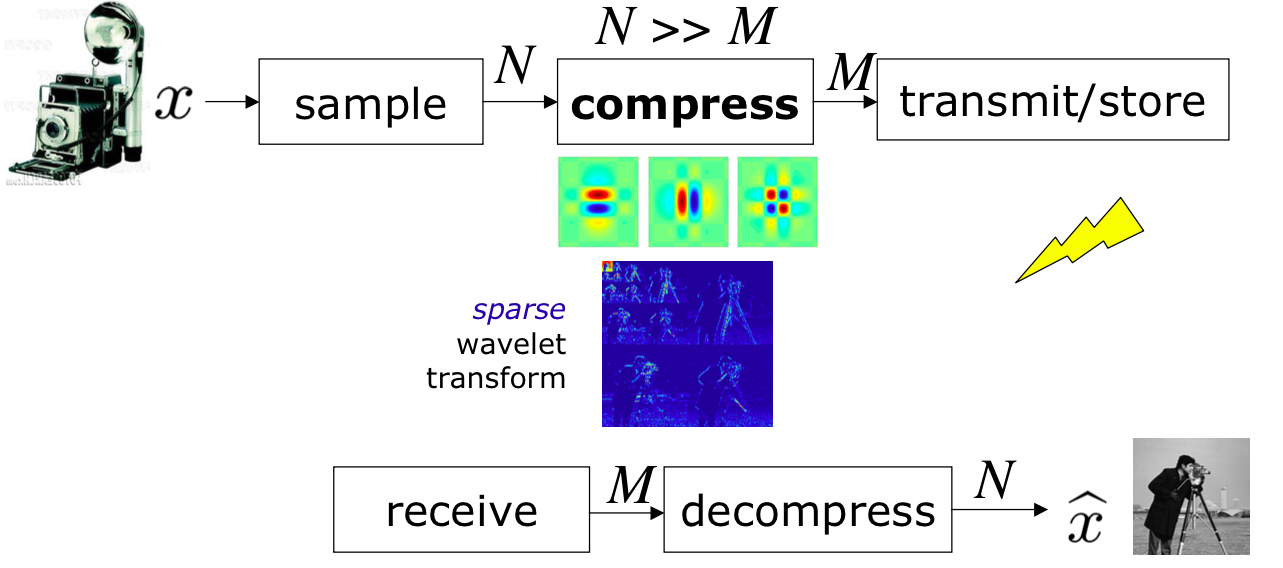
\includegraphics[width=5.0in]{figs/wavelets-arch.png}
%\DeclareGraphicsExtensions.
%\caption{An example of wavelet compression procedure. The camera first samples the image, and then analyses it using wavelets to compress and transmit. At the receiving end, the image is reconstructed.}
%\end{figure}


%---- contributes topics ----

%In order to solve these problems, this report studies novel approaches which respectively embed the CS framework into those systems. In our proposed CS-UWB system, random projection is located at transmitters to support CS framework while sub-Nyquist low-rate ADCs are implemented at receivers. As a result, not only the accuracy is improved but also the sampling cost is significantly reduced. On the other hand, we study the recent CS-CSS systems' performance and analyize the cost of embedding CS into such systems. The analysis result indicates us that rather than fully reconstructing the CS measurements, the partial recovery or extraction useful information directly from unrecovered signals is more attractive and suitable in many cognitive radio spectrum sensing cases since it improves the real-time capability while keeps low sampling rate in CS. This idea intrigues our future research directions and motivations aiming at compressive signal processing (CSP, including compressive measurements analysis and partial support recovery etc) for wideband signal processing in cognitive radios and ultra wideband systems.

%---- contributes summary ----

%\paragraph{Compressive digital filter and estimation:} Following the idea that signal recovery is not actually necessary in many signal processing applications, we broaden this result and demonstrate that random measurements can universally capture the information relevant for many CSP applications without any prior knowledge of either the signal class or the ultimate signal processing task. For instance, in [xx], a circulated matrix based filter paradigm is mathematically proved, which can directly extract useful information from compressive measurements without recovery. This idea can be embedded in many filter-bank needed designs then eliminate the existence of analog filter while implement the filter in digital domain. In this way, complexity and power cost can be saved.

%The detection, estimation, and classification tools we develop in this paper enable the system to perform these tasks much more efficiently in the compressive domain. Furthermore, the filtering procedure we describe facilitates the separation of signals after they have been acquired in the compressive domain so that each signal can be processed by the appropriate algorithm, depend- ing on the information sought by the user. 

\chapter{Compressed Sensing and Low Rate ADC}\label{C:compressed_sensing}
\indent \indent In this chapter, we first introduce basic compressed sensing (CS) theory including sparse representation, incoherence, and reconstruction. Then we focus on how to build CS based ADC architectures, and presents our survey work for recent CS-ADCs. This work establish a good preparation for future CS  applications for wireless devices. Later on, some general hardware architectures for CS reconstruction and processing are introduced. At last, a brief introduction of future CS application for wireless communication is presented.

\section{Introduction}
\indent \indent In today's big data era, signal processing devices are always perplexed by its heavy power and storage cost due to the size and sampling requirements. The sampling requirements are mainly due to the Shannon sampling theory which states that the minimum sampling rate should be at least twice as the most highest frequency components in original signal (we call it the Nyquist rate). As a fact, the limitation in signal sampling not only increases the design complexity to analog-to-digital converters (ADCs), but increases the data size of storage, as well as the scale for further data processing. Consequently, the power consumption, computational cost, and commercial design cost become raising. What's worse, if we cannot solve the sampling limitation, then not only sampling itself, which relates to faster sampling, larger range and sensing mobility, but also burden storage for high dimensional data and energy saving for low-energy consumption, will be significantly affected. In conclusion, all requirement refers to the key problem of sampling. From this aspect, solving the limitation in signal sampling is by no means tolerable for modern signal processing devices.

Since acquisition approach is crucial, many recent researches aim at how to select useful interest of signals more efficiently. Examples such as wavelet \cite{chui1992introduction} have significantly reduced the compressed size, and extracted very sparse information from original data. However, before we can extract such interests, the Nyquist rate of sampling is STILL required, thus the heavy burden in ADCs could NOT be neglected. In other words, the limitation from Nyquist rate does not eliminated for hardware devices.  

Fortunately, the compressed sensing (CS) presents us an useful alternative to extract sparse interests of signal BELOW Nyquist rate \cite{lustig2008compressed}. The CS framework provide high possibility to reconstruct original signals through randomly sampled measurements, and the sampling rate is far below the Nyquist rate.As a result, the CS framework is becoming popular in many high frequency or wideband signal acquisition required systems and devices. 

\section{Compressed Sensing Theory}\label{sct:cs_theory}
\indent \indent This section mainly introduces the theory in compressed sensing. 

\subsection{Compressed Sensing Paradigm}\label{sct:cs_paradigm}
\indent \indent Compressed sensing (CS) announces that sparse informations can always be reconstructed from far fewer samples than traditional method of Nyquist Theorem. Assume the sensing system is $y = \Phi x$, where $y \in R^m$ is the observation, $\Phi_{m \times N}$ is the sensing matrix, and $x \in R^N$ is the original signal to be reconstructed. Here $m << N$ which implies the sampling rate is relatively low. The following paragraphs in this section briefly introduce the CS framework.

\paragraph{Sparse representation}
Consider a task of sampling a signal of $x$ using sub-Nyquist rate. Suppose that a group of basis $\Psi$ provides a $K$-sparse representation of signal $x$ as following, where $k << N$.
\begin{equation}
\label{eq_sparse}
x=\Psi s=\sum_{l=1}^{K}\psi_l s_l  
\end{equation}
Here $x$ is a linear combination of $K$ basis chosen from $\Psi$, and $s$ is the corresponding coefficients of representing $x$ in the domain constructed by the basis $\Psi$. 
%re-wr begin{6126712

\paragraph{Reconstruction}
Then Candès, Romberg and Tao \cite{candes2006robust} showed that one could almost always recover the signal $x$ exactly by solving the following $l1$-norm minimisation problem (convex program, equation \ref{eq_bp}):
\begin{equation}
\label{eq_bp}
\hat s = \arg\min \| s \|_1 \quad s.t. \quad  y = \Phi \Psi s
\end{equation} 
\begin{theorem}\label{thm_bp}
This formulation is known as basis pursuit (BP). Assume that $x$ is $K$-sparse and we are given $m$ Fourier coefficients with frequencies selected uniformly at random. Suppose that the number of observations obeys
\begin{equation}
\label{eq_observation}
m \leq C \cdot K \cdot log N 
\end{equation} 
Then minimizing $l1$ reconstructs $x$ exactly with overwhelming probability which exceeds $1 − O(N^\delta)$.
\end{theorem}
Further, reconstruction from noisy measurements can be stated in a relaxed form as a basis pursuit de-noising (BPDN) \cite{chen1998atomic} problem, which allows some measurement mismatch of $\epsilon > 0$: 
\begin{equation}
\label{eq_bpdn}
\hat s = \arg\min \| s \|_1 \quad s.t. \quad  \| y - \Phi \Psi s \|_2 \leq \epsilon
\end{equation} 

\paragraph{Restricted Isometry Property}
We also need means to quantify the robustness of CS under noisy and only approximately sparse conditions. The most prominent criterion for is the restricted isometry property (RIP) in \cite{candes2005decoding}. This property essentially requires that every set of columns of the sensing matrix behaves like an orthonormal system. Namely, the RIP measures how well distances are preserved in a linear transformation. A matrix $A$ fulfills the RIP with restricted isometry constant $\delta_K$ if
\begin{equation}
\label{eqn_rip1}
(1-\delta_k) \| s \|_2 \leq A s \leq (1+\delta_k) \| s \|_2
\end{equation}
Cand´es et al. \cite{candes2006stable} introduces an error bound for the solution of BPDN equation \ref{eq_bpdn} under the condition that $\delta_{3K} + 3 \delta_{4K} < 2$ and that the error $\|e\|_2 < \epsilon$:
\begin{equation}
\label{cs_error_bound}
\| x - \hat x \|_2 \leq C_1 \epsilon + C_2 \delta_K (x)_1 / \sqrt{K} 
\end{equation}
where the C1 and C2 are small constant, and $\delta_K (x)_1$ is the minimal $l1$-error introduced by the best possible $K$-sparse approximation. 

\paragraph{Incoherence}
A criterion related to the RIP is the incoherence of the projection $\Phi$ and the sparsifying basis $\Psi$. The mutual coherence is defined as:  
\begin{equation}
\label{cs_coherent}
\mu (\Phi, \Psi) = \max_{i \in [1,m]; j \in [1,N]} | < \phi_i, \psi_j > | 
\end{equation} 
The less coherent the two matrix $\Phi$ and $\Psi$ are, the better the reconstruction works. The greater the incoherence of the measurement/sparsity pair $(\Phi, \Psi)$, the smaller the number of measurements needed.
%re-wr end 6126712}

\paragraph{Sensing Matrix}
In order to successfully recover the $s$, we have to compose and construct sensing matrix $A$ by $\Phi$ and $Psi$ to satisfy the RIP. However, calculating the restricted isometry constant of a given matrix $A$ is itself a problem of combinatorial complexity. Hence, artificially designing and testing the RIP of a sensing matrix is difficult. Fortunately, random variable composed matrix, whose entries are independent and identically distributed (i.i.d) variables, are very likely satisfies the requirements\cite{rauhut2010compressive}. Besides, if the projection matrix $\Phi$'s variables are i.i.d and basis matrix $\Psi$ is Fourier, or wavelets alike matrix, then the overall sensing matrix $A = \Phi \Psi$ still keeps high probability to achieve a successful recovery (similar to the conclusion in theorem \ref{thm_bp}). What's more, as long as the incoherence of $\Phi$ and $\Psi$ great enough, exactly reconstruction from equation \ref{eq_bpdn} is possible. As researches in projection matrix $\Phi$ develops, sub-Gaussian distribution measurement, Bernoulli measurement, random partial Fourier measurement, random Toeplitz measurement\cite{bajwa2007toeplitz} are all proven suitable for CS sampling and reconstruction, and widely used for constructing the measurement in CS applications. 
 
\subsection{Reconstruction Algorithms}
\indent \indent The $l1$-minimization plays an important role in successfully designing computationally stable CS reconstruction. This approach can be treated as convex optimization such as basis pursuit\cite{chen1998atomic} and Bregman\cite{yin2008bregman}. However, although they recover signal with lower average error, but they are computationally burdensome. On the other hand, some other sort of algorithms recover sparse signal termed combinatorial algorithms including chaining pursuit\cite{gilbert2006algorithmic} and HHS pursuit\cite{gilbert2007one} can achieve extremely rapid computational speed for sparse signal reconstruction but seems to be sensitive to noise as they strongly rely on the group testing of highly structured samples.
 
Compared to convex optimization and combinatorial algorithms, greedy pursuit algorithms particularly are intermediate of the fast running time and sampling efficiency, and become a better trade-off between speed, stability and robustness. Popular greedy pursuits include OMP\cite{pati1993orthogonal}, CoSaMP\cite{needell2009cosamp}, HTP\cite{blumensath2009iterative} etc. In recent CS based signal acquisition and reconstruction systems where both time saving and recovery precision are crucial, hence greedy pursuits are widely utilized. The following subsections introduces prevailing greedy pursuit algorithms. 

\paragraph{Orthogonal Matching Pursuit}
Orthogonal matching Pursuit (OMP)\cite{mallat1993matching} is a widely used for sparse reconstruction which develops the process of matching pursuit. As shown in algorithm \ref{OMP}, it progressively manages to find the support of the unknown sparse signal: Give an acquisition system $y = As$ where $s \in R^N$ is $K$ sparse and CS measurement $A \in R^{m \times N}$ $(m << N)$, each iteration of OMP selects one support $\lambda$ of the vector $s$ which contributes the most to the observation $y$. This selection method is based on testing the correlation values between the current columns of $A$ and residue $r$. The OMP iteration would not stop before the residue $r$ becomes relatively small. 

\IncMargin{1em}
\begin{algorithm}
    \SetKwData{Left}{left}\SetKwData{This}{this}\SetKwData{Up}{up}
    \SetKwFunction{Union}{Union}\SetKwFunction{FindCompress}{FindCompress}
    \SetKwInOut{Input}{input}\SetKwInOut{Output}{output}
    \Input{measurement $A \in R^{m \times N}$, observation $y$.}
    \Output{recovery $\hat s$.}
    \BlankLine
	$r_0 \gets y$; $\Lambda_0 \gets \Theta$; $i \gets 0$; \;
	\While {$r_i \geq theshold$}{
		$h_i \gets A^T r_i$ $\quad //match$\;
		$\Lambda_{i+1} \gets \Lambda_i \cup \{\arg\max_{1 \leq j \leq N} |h_i(j)|\}$ $\quad //identity$\; 
		$ \hat s_{i+1} \gets \arg\min_s \|y-A_{\Lambda_{i+1}} \hat s_i\|_2$ $\quad //determine$\; 
		$r_{i+1} \gets y - A\hat s_{i+1}$ $\quad //update$\;
	}
\caption{Orthogonal Matching Pursuit(OMP)}\label{OMP}
\end{algorithm}
\DecMargin{1em}

The computational complexity of OMP is $O(KmN)$ which is significantly smaller compared to classical convex optimization such as basis pursuit whose complexity is $O(N^3)$ (in case that sparsity of $K << N$)\cite{dai2009subspace}. However, the robustness of OMP cannot reach the quality level of traditional convex optimization, since searching local optimal solutions instead of global solutions brings more errors to OMP.  

\paragraph{Compressed Sensing Matching Pursuit}
In order to improve the speed and robustness of OMP, Compressed Sensing Matching Pursuit (CoSaMP)\cite{needell2009cosamp} is developed. It aims at producing a more effective way for detecting the support of input signals shown in \ref{CoSaMP}: The CoSaMP firstly find $2K$ indices for maximal correlation between columns of $A$ and the current residue $r$ by using the operator $H_{2K}(A^T r)$ to set all but the $2K$ largest components in $A^T r$ to zero. Then CoSaMP merges these $2K$ indices with the previous support from current recovered $\hat s$, in order to form a new support set $\lambda$ for updating the least square solution of $\hat s$. In the next step, the least squares solution is pruned and consequently only the $K$ largest components are preserved.  

\IncMargin{1em}
\begin{algorithm}
    \SetKwData{Left}{left}\SetKwData{This}{this}\SetKwData{Up}{up}
    \SetKwFunction{Union}{Union}\SetKwFunction{FindCompress}{FindCompress}
    \SetKwInOut{Input}{input}\SetKwInOut{Output}{output}
	\Input {measurement $A \in R^{m \times N}$, observation $y$, sparsity $K$.}
	\Output{recovery $\hat s$.}
    \BlankLine
	$r_0 \gets y$; $i \gets 0$. \;
	\While {$stopping \; the \; criterion$}{
		$h_i \gets H_{2K}(A^T r_i)$  $\quad //match$ \; 
		$\Lambda \gets supp(h_i) \cup supp(\hat s_i)$ $\quad //identity$ \;
		$\hat s_{i+1} \gets \arg\min_s \|y-A_{\Lambda} \hat s_i\|_2$ $\quad //determine$ \;
		$(s_{i+1})_j \gets 0 \; for \; j \not\in \Lambda_i$ \;
		$r_{i+1} \gets y - A\hat s_{i+1}$ $\quad //update$  \;
	}
\caption{Compressed Sensing Matching Pursuit(CoSaMP)}\label{CoSaMP}
\end{algorithm}
\DecMargin{1em}

Although other revised matching pursuits such as ROMP\cite{needell2009uniform}, StOMP\cite{donoho2006sparse} have been developed for improving the robustness of OMP. However, compared to those revise for OMP, CoSaMP offers the optimal performance as it works with a minimal number of observations and performs a better recovery robustness to noise \cite{needell2009cosamp}.

\paragraph{Hard Thresholding Pursuit(HTP)}
Similar to CoSaMP, HTP enhances the stability and robustness by improving the efficiency for detecting the support set $\Lambda$ from obeservation $y$, through considering larger range of correlations between residues $r$ and measurement $A$\cite{foucart2011hard}. In this algorithm, each iteration of HTP performs a gradient descent aiming at the final solution in order to estimate $k$ supports that contributes most to the observation $y$. Next, by solving a pruned least squares problem, HTP updates its solution $\hat s$ and residue $r$ for the next iteration. The pesudocode of the algorithm is given in \ref{HTP}: 

\IncMargin{1em}
\begin{algorithm}
    \SetKwData{Left}{left}\SetKwData{This}{this}\SetKwData{Up}{up}
    \SetKwFunction{Union}{Union}\SetKwFunction{FindCompress}{FindCompress}
    \SetKwInOut{Input}{input}\SetKwInOut{Output}{output}
	\Input {measurement $A \in R^{m \times N}$, observation $y$, step size $v$, sparsity $K$.}
	\Output{recovery $\hat s$.}
    \BlankLine
	$r_0 \gets y$; $i \gets 0$. \;
	\While {$stopping \; the \; criterion$}{
		$h_i \gets \hat s_i + v A^T r_i$ $\quad //gradient decent$ \;
		$\Lambda \gets supp(H_k(h_i))$ $\quad //identity$ \;
		$\hat s_{i+1} \gets \arg\min_s \|y-A_{\Lambda} \hat s_i\|_2$ $\quad //determine$ \;
		$(s_{i+1})_j \gets 0 \; for \; j \not\in \Lambda_i$ \;
		$r_{i+1} \gets y - A\hat s_{i+1}$ $\quad //update$ \;
	}
\caption{Hard Thresholding Pursuit(HTP)}\label{HTP}
\end{algorithm}
\DecMargin{1em}

\subsection{Performance of Greedy Pursuits}
\indent \indent Among the prevailing greedy pursuit algorithms of OMP, ROMP, StOMP, CoSaMP, HTP, the CoSaMP and HTP outperform other greedy pursuits in terms of stability\cite{foucart2011hard}. In addition, according to \cite{blumensath2009use}, by comparing the output Signal-to-Noise(SNR) in recovered sparse signals, it suggests that average SNR provided by CoSaMP and HTP are approximately very close to the traditional BP, which indicates that revised greedy pursuits such as CoSaMP finally reach the high quality level of robustness provided by the classical convex optimizations. Besides, most of the greedy pursuit algorithms remain lower computational complexity than convex optimizations. For instance, the complexity of ROMP, StOMP, CoSaMP and HTP are $O(KmN)$, $O(N \ln N)$, $O(mN)$ and $O(MN)$respectively, and all surpass that in convex algorithms such as BP ($O(N^3)$)\cite{qaisar2013compressive}. In conclusion, the revised greedy pursuits preserves the fast speed of its own, and successfully develops higher stability and robustness. Consequently, they become suitable and widely implemented in CS applications involved fast sparse reconstructions.  

\section{Compressive ADC Architectures}
\indent \indent Analog-to-Digital converter (ADC) is utilized in many consumer electronics products that interact with real-world signals which are predominantly analog in nature. The conversion of the analog signals involves the sampling process has long been bounded by the Nyquist theory which declares the minimum sampling rate for traditional acquisition methods, and couldn't reduced easily. In order to overcome this problem, recently many signal processing devices embed CS into analog-to-digital converters(ADCs) and successfully reduces the size of measurements and thus releases the limitation given by the Nyquist theory. As a consequence, the new systems using a relatively lower clock rate significantly outperform the traditional acquisition systems.   

\subsection{Random Demodulator}
\indent \indent Random demodulator (RD) \cite{tropp2010beyond} is one of the most popular analog-to-digital converters for CS-based signal acquisition and processing. It develops the stability and robustness of CS measurement, and achieves a sub-Nyquist rate ADC for signal sampling and sequentially enhances the system power efficiency (especially the performance of front-end acquisition systems).  

\begin{figure}
\centering
\includegraphics[width=0.5\columnwidth]{figs/random_demodulator.pdf}
\DeclareGraphicsExtensions.
\caption{Block diagram of random demodulator (RD). The components includes a pseudo-random sign generator, a low-pass filter, and a sub-Nyquist ADC}\label{RD}
\end{figure}

Figure \ref{RD} shows the construction of the random demodulator: The $K$-sparse input signal $x$ is first mixed with the chipping sequence $p_c(t)$ which is a waveform constructed by pseudo-random variables of $\{\pm 1\}$. The mixed product component $x(t) \cdot pc(t)$ is then passed through an anti-aliasing low pass filter h(t), before being sampled at a uniform interval but at a lower sampling rate of m which is of the order $(K log(N/K))$ which is much lower than the normal required rate corresponds to $N$ (since $K << N$). The most widely used reconstruction algorithms for RD are those based on OMP and CoSaMP greedy pursuit. Experimental results \cite{tropp2010beyond} demonstrates that the minimal sampling rate needed is only $1.7K(log(N/K))$ and in addition, it provides better SNR performance when compared with conventional Nyquist rate based ADCs.

\subsection{Modulated Wideband Convertor}
\indent \indent In the cases of sampling a multi-band signals whose carrier frequencies are unknown or time-variant (blind multi-band signal receiving), the main task is to design a receiver working independently on the carrier frequency at a low rate \cite{mishali2009blind}. Recently, a novel architecture termed modulated wideband converter (MWC) is developed, which applies the CS theory to the traditional blind multi-band signal receivers based on non-uniform sampling\cite{black1980time}. This innovative architecture successfully provides a minimal requirement for the size of observations \cite{mishali2010theory} thus decrease the power consumption. Besides, compared to the RD, MWC provides robustness against the noise and model mismatches.

The MWC consists of groups of periodic waveforms, low pass filters and sub-Nyquist rate ADCs, and can be treated as a parallel structure of the random demodulator (RD). As shown in Figure \ref{MWC1}, each group of periodic sequence $p_i(t)$ with minimum interval of $T_p/M$ mixes the input multi-band signal $x(t)$ for shifting the spectrum by $\Delta f_p$ ($f_p = 1/{T_p}$ is the frequency of $p_i(t)$) and filtering it to the baseband for sampling. In the end, low rate ADCs sample the mixed productions at a rate $f_s$ far less than the Nyquist rate $f_{NYQ}$.
\begin{figure}
\centering
\includegraphics[width=0.5\columnwidth]{figs/MWC1.pdf}
\DeclareGraphicsExtensions.
\caption{Block diagram of modulated wideband convertor (MWC). The components includes parallel periodic waveforms mixers, low-pass filters, and sub-Nyquist ADCs}\label{MWC1}
\end{figure}

Reconstruction is done by subspace detection via continuous to finite block (CTF) \cite{mishali2009blind}. The CTF block is comprised of frame construction, and the multiple measurement vectors (MMV) that can be solved by greedy pursuits based algorithms. The signal reconstruction can be achieved by a direct pseudo-inverse operation based on results of the CTF block.

\subsection{Non-Uniform Sampling}
\indent \indent Apart from the modulated based CS architectures such as random demodulators and modulated wideband converters which uniformly samples the mixed input analog signals at a slow rate, another novel CS architecture -- the non-uniform sampling which is based on the theory of information recovery from random samples \cite{ragheb2007implementation} develops recently. This architecture aims at sampling signals in a local Fourier sparse representation\cite{rauhut2010compressive} (LFS) (e.g. wideband signals), and provides an non-uniformly sampling pattern at pseudo-random time points with a low average rate. An example of this sampling pattern is shown in Figure \ref{RS-ADC}. 
\begin{figure}
\centering
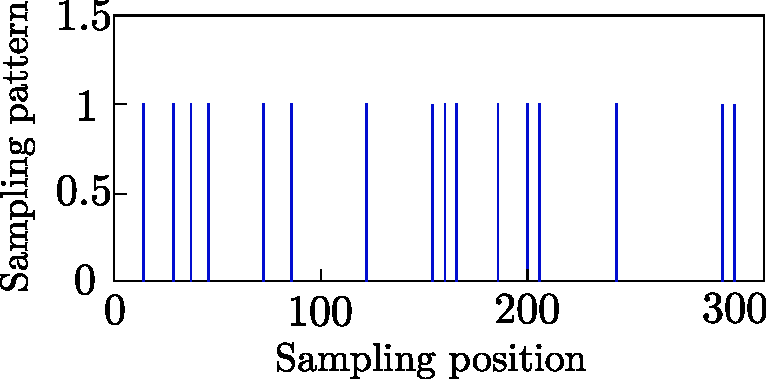
\includegraphics[width=2.6 in]{figs/NUS.pdf}
\DeclareGraphicsExtensions.
\caption{A pseudo-randomly sample pattern for single pure tone signal of length 300}\label{NUS}
\end{figure}

The matrix multiplication between $F$ and $s$ stands for the input signal $x$ which contains sparse spectrum $s$, and $F$ is the full discrete time Fourier transform (DFT) matrix. The diagonal matrix $D$ represents the behavior of non-uniform sampling, where the value $\epsilon$ of diagonal items are chosen pseudo-randomly from $\{0,1\}$. 

The NUS based CS acquisition model establishes a sensing matrix $A$ which equal $DF$ and can be regarded as a random partial Fourier matrix $F_{T}$ which consists of randomly chosen columns of the discrete Fourier matrix (DFT) and indexed by $T$. According to \cite{ragheb2007implementation}, the matrix $A$ satisfies the RIP in compressive sensing so the acquisition model produces a stable reconstruction of $\hat s$ via $l1$-minimisation using $m \geq O(slog(N/s))$ samples\cite{ragheb2007implementation}. In addition, many greedy algorithms such as OMP and CoSaMP are also implemented as fast reconstruction for this architecture \cite{maechler2011random}.

\subsection{Compressive Multiplexer}
\indent \indent Common implementations of the CS based non-uniform sampling architectures varies from \cite{laska2006random, ragheb2007implementation, maechler2011random, rogers2011compressive}. Among these implementations, the random sampling compressive sensing ADC (RS-ADC) is likely to be the prevailing design shown in Figure \ref{RS-ADC}. This architecture is comprised of input multiplexers (MUX), analog queues (AQs), demultiplexer (DEMUX) and a low-rate successive ADC. 
\begin{figure}
\centering
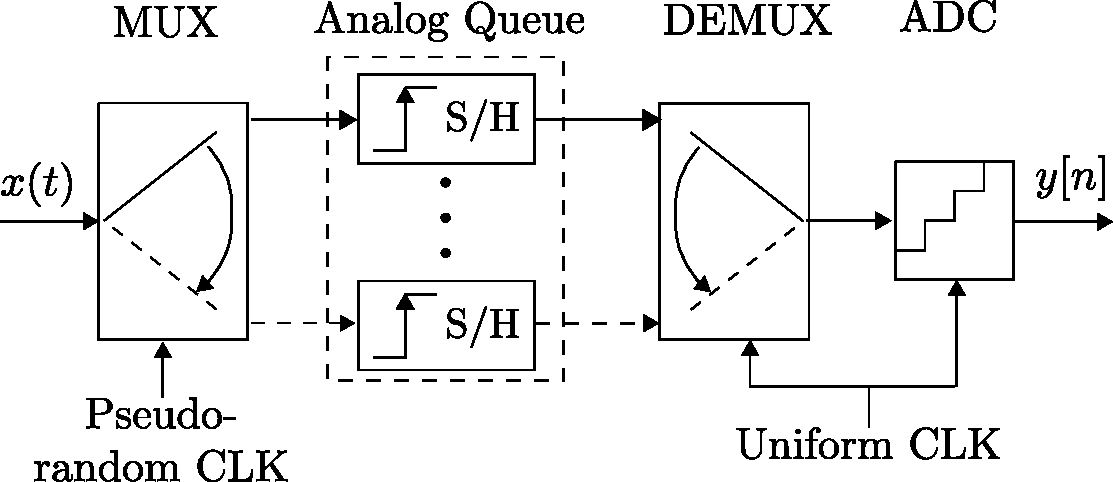
\includegraphics[width=3.0in]{figs/RSADC.pdf}
\DeclareGraphicsExtensions.
\caption{Block diagram of the random sampling CS ADC (RS-ADC). The components includes a pseudo-random sign generator, a low-pass filter, and a sub-Nyquist ADC}\label{RS-ADC}
\end{figure}

This implementation uses an input multiplexer driven by a non-uniform clock to switch the signal among several parallel $S/H$ based analog queues. A low rate ADC (e.g. Successive Approximation ADC) is used to convert the stored samples, performing at uniform intervals but operating at sub-Nyquist average rate. Greedy pursuit algorithms such as OMP and CoSaMP are then used to perform fast reconstruction for this architecture. However, the main problem of applying RS- ADC lies in sampling high frequency signals: since the ADC and input MUX perform inherent bandwidth limitations modeled as a lowpass filter preceding the uniform sampling, acquisitions for high frequency signals results in a loss of the spectrum components. Besides, the high switching speed of the MUX increases noise and reduces the power efficiency.

\section{Conclusion}\label{sct:cs_conclusion}
\indent \indent The Nyquist sampling theorem states that signal should be sampled at least two times faster than the signal bandwidth so that the aliasing would not occur. However, modern applications produce a large amount of data, resulting in large numbers of samples which requires high speed sampling. To overcome this problem, the compressive ADC architectures are studied in this chapter. First we present the theory of CS framework, then a comprehensive survey of the novel compressive ADC (CS-ADC) designs are studied. Major types of CS-ADCs, such as random demodulators, modulated wideband converters, non-uniform samplers, and compressive multiplexer are explained in detail. 

%--------------------------------------------------------------

%\section{Related Works: Sub-Nyquist Analog-to-Digital Convertor}\label{sct:sub-nyquist_adc}
%\indent \indent Compressed Sensing (CS) is a technique XXX
%%cs-rd_intro.tex
\subsection{Wideband Compressed Sensing ADCs}\label{sct:wideband_cs_adc}
Sampling rate is crucial to signal processing systems since high clock rate enhances the power consumption and increases the burden of data transmission and storage. However, it has long been bounded by the Nyquist theory which denotes the minimum sampling rate for traditional acquisition methods, and couldn't reduced easily. In order to overcome this problem, recently many signal processing devices embed CS into analog-to-digital converters (ADCs) and successfully reduces the size of measurements and thus releases the limitation given by the Nyquist theory. As a consequence, the new systems using a relatively lower clock rate significantly outperform the traditional acquisition systems.   

\subsubsection{Random demodulator}
Random demodulator (RD)\cite{tropp2010beyond} is one of the most popular analog-to-digital converters for CS-based signal acquisition and processing. It develops the stability and robustness of CS measurement, and achieves a sub-Nyquist rate ADC for signal sampling and sequentially enhances the system power efficiency.  

\begin{figure}[!b]
\centering
\includegraphics[width=3.2in]{pictures/random_demodulator.pdf}
\DeclareGraphicsExtensions.
\caption{Block diagram of random demodulator (RD). The components includes a pseudo-random sign generator, a low-pass filter, and a sub-Nyquist ADC}\label{RD}
\end{figure}

Figure \ref{RD} shows the construction of the random demodulator: It consists of a pseudo-random sign generator, a low-pass filter, and a sub-Nyquist ADC. The input $K$ sparse signal is first mixed with the chipping sequence $p_c(t)$ which is a waveform and constructed by pseudo-random variables of $\{\pm 1\}$. This chipping sequence is generated by the pseudo-random sign generator which alternates at the Nyquist rate $N$. The mixed production $x(t) \cdot p_c(t)$ then passes through a low pass filter $h(t)$ for anti-aliasing, and finally is sampled by a ADC uniformly at the rate of $m = O(K\log(N/K)) << N$. %N = W , R = M

\subsubsection{Modulated Wideband Convertor}
In the cases of sampling a multi-band signals whose carrier frequencies are unknown or time-variant (blind multi-band signal receiving), the main task is to design a receiver working independently on the carrier frequency at a low rate\cite{mishali2009blind}. Recently, a novel architecture termed modulated wideband converter (MWC) is developed, which applies the CS theory to the traditional blind multi-band signal receivers based on non-uniform sampling\cite{black1980time}. This innovative architecture successfully provides a minimal requirement for the size of observations\cite{mishali2010theory} thus decrease the power consumption.

\begin{figure}[!t]
\centering
\includegraphics[width=3.2in]{pictures/MWC1.pdf}
\DeclareGraphicsExtensions.
\caption{Block diagram of modulated wideband convertor (MWC). The components includes parallel periodic waveforms mixers, low-pass filters, and sub-Nyquist ADCs}\label{MWC1}
\end{figure}

The MWC consists of groups of periodic waveforms, low pass filters and sub-Nyquist rate ADCs, and can be treated as a parallel structure of the random demodulator (RD). As shown in Figure \ref{MWC1}, each group of periodic sequence $p_i(t)$ with minimum interval of $T_p/M$ mixes the input multi-band signal $x(t)$ for shifting the spectrum by $\Delta f_p$ ($f_p = 1/{T_p}$ is the frequency of $p_i(t)$) and filtering it to the baseband for sampling. In the end, low rate ADCs sample the mixed productions at a rate $f_s$ far less than the Nyquist rate $f_{NYQ}$.

Considering the CS measurement MWC, recovering the $\mathbf z(f)$ where each row $X(f-lf_p)$ presents sparse spectrum segments can be regarded as recovering a infinite set of joint sparse vectors. This problem can be solved by changing it to the problem of multiple measurement vectors (MMV)\cite{mishali2008reduce} and has been implemented. 

\subsubsection{CS based signal processing}
Considering that many signal processing applications such as detection, classification, estimation and filtering do not require entire signal reconstruction, and only parts of certain information from measurements are needed, thus we prefer to filter out the useless information before further signal processing. Therefore, if we could estimate the useless information corresponding to some observations $y_I$, and then $throw$ them $away$ before CS based signal recovery, we can avoid a high computational complexity and thus save the power efficiency significantly. This novel idea comes from the compressive signal processing (CSP)\cite{davenport2010signal}.

\subsubsection{Non-Uniform Sampling}
The non-uniform sampling aims at sampling signals in a local Fourier sparse representation\cite{rauhut2010compressive} (LFS) (e.g. wideband signals), and provides an non-uniformly sampling pattern at pseudo-random time points with a low average rate, which establishes a sensing matrix $A$ which can be regarded as a random partial Fourier matrix $F_{T}$ that consists of randomly chosen columns of the discrete Fourier matrix(DFT) and indexed by $T$. According to \cite{ragheb2007implementation}, the matrix $A$ satisfies the RIP in compressive sensing so the acquisition model produces a stable reconstruction of $\hat s$ via $l1$-minimization using $m \geq O(slog(N/s))$ samples\cite{ragheb2007implementation}. 

%\indent \indent 

%--------------------------------------------------------------

%\section{Reconstruction Architecture}\label{sct:imple_fast_recon}

%Impressive progress has been made in fast decades for compressed sensing and its applications. However, the reconstruction for compressive measurements always need long-time execution if accurate and robust results are required, e.g. basis pursuit requires $O(N^3)$ running time which far larger than $O(kmn)$ in algorithms like orthogonal matching pursuit in \ref{omp}. 

%In other words, computational efforts for high performance recovery of compressive measurements are still difficult and crucial. In this section, some general matching pursuit based recovery architectures are introduced, and the motivation of compressive signal processing (CSP) is mentioned.

%However, the computational effort for successful signal recovery remains high, even for problems of moderate size. Reconstruction becomes especially challenging for real-time applications with stringent power constraints, e.g., on mobile devices. Such applications require efficient hardware implementations of sparse signal recovery algorithms, which we develop in this thesis. We present different architectures of greedy algorithms for a number of selected applications. The first example is the estimation of sparse channels in broad-band wireless communication. The use of sparse recovery algorithms efficiently reduces noise and, thus, increases estimation quality. Architectures for three algorithms are developed and their realisations. in application-specific integrated circuits (ASICs) are compared. We show that approximative algorithms deliver good results at low hard- ware complexity. The second application is the recovery of signals corrupted by structured noise. Using the example of audio restoration from corruptions by clicks and pops, fast realisations of the approximate message passing algorithm are designed. Two fundamentally different architectures —one relying on fast transforms, the other relying on parallel processing power—are developed and compared. Large gains in terms of throughput and circuit complexity are realised by applying fast transforms in the context of CS recovery. The choice of the most attractive algorithms and architectures depends on the sparsity, the number of measurements, and the basis in which the samples are taken. In general, approximate message passing is found to be very well suited for hardware recovery of moderately sparse signals while serial greedy pursuits are better suited for very sparse signals.
%} 

%------------
% parallel ..
% hardware OMP. 
% AMP ..
% CoSaMP
%------------

%re-wr{
%The introduction of compressive sensing (CS) led to a new paradigm in signal processing. Traditionally, signals are sampled above their Nyquist rate. Using CS, the same information is acquired with much fewer measurements, provided a sparse representation of the signal exists. This makes CS a very promising technology with a large number of potential applications.
%While the acquisition of measurements is simplified, the reconstruction of the original signal becomes more involved. Sparse signal recovery algorithms solve the corresponding systems of underdetermined linear equations and have proven very efficient for various applications. 
%Examples include de-noising, the restoration of corrupted signals, signal separation, super-resolution, and in-painting. All applications are based on the observation that many natural and man-made signals have sparse representations in some suitable bases.
%}
%In this chapter, we give a review of the theory of compressed sensing system. In addition, the typical applications in radar system and medical scanners (e.g. magnetic resonance imaging, MRI) are introduced. Moreover, we focus on our related work for a survey of potential analog-to-digital convertors for future wireless devices.
%------


%----description of CS-MUX ----
%The workflow of RS-ADC can be described as the following steps: At first, it orderly dispatched the input analog signal through a multiplexer which is driven by a non-uniform clock. Then, the system store the dispatched analog signal in different analog queues using sample and hold (S/H). At last, the demultiplexer driven by a periodic clock sequentially selects the output of the analog queue and transfers the value to the low-rate ADC. Considering the modulated based CS-ADC such as the RD and MWC, the NUS such as RS-ADC is an alternative architecture to establish a constructed pseudo-random measurement for CS based ADC design. Compared to the RD and MWC, the advantage of RS-ADC stays in the fact that it saves power consumption and chip area since it doesn’t need to mix a high rate chipping sequence and only contains a single ADC. However, the main drawback of the NUS is obvious non-idealism caused by the timing jitter. The timing jitter, which derives from the input multiplexer, brings sample error and propagates it through the entire system thus produces additional noise and critical inaccuracy. Moreover, switch capacitors and delay in multiplexers also reduces the robustness of the RS-ADC systems. 


% ---- desciption of RD -----
%It consists of a pseudo-random sign generator, a low-pass filter, and a sub-Nyquist ADC. The input $K$ sparse signal is first mixed with the chipping sequence $p_c(t)$ which is a waveform and constructed by pseudo-random variables of $\{\pm 1\}$. This chipping sequence is generated by the pseudo-random sign generator which alternates at the Nyquist rate $N$. The mixed production $x(t) \cdot p_c(t)$ then passes through a low pass filter $h(t)$ for anti-aliasing, and finally is sampled by a ADC uniformly at the rate of $m = O(K\log(N/K)) << N$. This design is simple, but easily affected by model mismatches and design imperfections.

\chapter{Compressive UWB Positioning}\label{C:compressive_uwb_positioning}
\indent \indent In this chapter, we first present an overview of UWB communication, and then focus on on our related work in Impulse-radio ultra-wideband (UWB) positioning system. The proposed work shows the potential advantages if we implement CS projection in the transmitter of the UWB positioning system according to the experiment result. Besides, Our proposed compressive UWB positioning presents a novel view of energy trade-off design, which is implemented by a low-rate random-projection at transmitters and low rate ADCs at receivers. It is clear that this design significantly reduce the peak frequency in the system with acceptable rate increase in receivers' ADC sampling rate.   

\section{Introduction}
\indent \indent Ultra-wide band (UWB) communication is widely used in wireless communication and associated with features as extreme wide transmission bandwidth, low-power consumption, shared spectrum resources in wide ranges etc \cite{paredes2007ultra}. Among all applicable areas, UWB based accurate positioning and tracking in short range communication become popular since it provides resilient to multipath fading in hostile environment and outstanding robustness even in low signal-to-noise (SNR) situations \cite{cassioli2002ultra}. In addition, the requirements of high data rate and limitations of battery supply lead the impulse-radio ultra-wide band (IR-UWB) to become a suitable communication technique in short range high data rate communication. As a result, applications based short-distance wireless sensor networks (WSNs) where large numbers of portable instrument, are widely deployed such as indoor positioning, surveillance, home automation, etc. 

However, high data rate transmission puts huge pressure on signal detection at ADCs at receivers, which indicates the sampling rate becomes a main bottleneck to the IR-UWB system. This paper focuses on the IR-UWB indoor positioning, aims at solving the bottleneck of sampling rate by using a recent novel technique termed compressed sensing (CS), aforementioned in Chapter \ref{C:compressed_sensing}. Compressed sensing is a novel paradigm which applies randomly sampling and sparse reconstruction, which enables a possible reconstruction strategy for sparse signals from a relatively small group of random measurements. It indicates that CS based IR-UWB systems can possibly detect high frequency sparse signals under a sub-Nyquist sampling rates that far below the Nyquist rate (twice the IR-UWB bandwidth). This result is advantageous which releases the bottleneck of the large bandwidth constraints on ADC at UWB receivers, and consequently reduces storage limits and improves energy efficiency in IR-UWB positioning systems.

Recently some researches manage to embed CS reconstruction algorithms, e.g. revised orthogonal matching pursuit, at UWB receivers. These algorithms successfully improve the SNR of the received signal before they are sent to the stages of time of arrival (TOA) based positioning algorithm. Consequently, this method increases the performance of entire positioning accuracy \cite{banitalebi2014compressive}. For hardware implementation of the new CS based UWB receivers, most of them apply the hardware structure termed the random demodulator (RD) \cite{kirolos2006analog}, and consequently this new CS-UWB receiver successfully reduces the sampling rate significantly compared to the Nyquist rate \cite{yang2011compressive}.

On the other hand, some researches embed the CS technique mainly at UWB transmitters. They develop a waveform-based precoding transmitter, in order to fulfil a random projection of the UWB generated pulses \cite{zhang2009compressed}. Followed by sub-Nyquist sampling ADCs at receivers, the sampled signals are sent to TOA based algorithm for calculating the location of the UWB transmitter. Simulation results show that the new CS-UWB transmitter manage to significantly decrease the sampling rate of receivers successfully improves accuracy of traditional UWB positioning system. 

However, both CS-UWB receivers and CS-UWB transmitters suffer from high-data rate random mixing operation, where PN sequence at mixers is required to reach the extremely high Nyquist rate ( e.g. beyond 10 GHz). This requirement generates heavy burden on bandwidth of hardware mixers and additionally increases a high frequency noise. To solve this problem, this paper propose an advanced low-rate CS-UWB positioning system: For the CS-UWB transmitter, it implements a relatively low-rate random projection matrix to slow down the mixing rate. For CS-UWB receivers, they sacrifices a small degree of compression ratio to keep equivalent performance as those positioning system using traditional CS-UWB transmitters. As a result, the trade-off between the random mixing rate and the sub-Nyquist sampling rate makes our system to become a more energy balanced, and consequently gains a better performance in entire power consumption and energy efficiency.  

\section{Model of Traditional UWB Positioning}
\indent \indent Extremely wide transmission bandwidths of the IR-UWB offers outstanding multipath resolutions for accurate positioning in indoor environment. Consider a typical UWB indoor communication model where distributed UWB receivers (base stations) are placed in an area to detect the location of a moving UWB transmitter (tag). The transmitter periodically broadcasts Gaussian shaped pulse $p(t)$ through an indoor multipath channel, and receivers detect signals for time of arrival (TOA) based positioning calculation. The received signals can be described as (\ref{eq_recv}):
\begin{equation}
\label{eq_recv}
r(t) = p(t) * h(t) + n(t) = \sum_{l=1}^{L} a_l p(t-\tau_l) + n(t) 
\end{equation}
where $p(t)$ is the transmitted Gaussian pulse, $n(t)$ stands for zero-mean additive white Gaussian noise (AWGN), and $h(t)$ refers to the standard UWB channel model denoted by IEEE 802.15.4a (\ref{eq_chan}):
\begin{equation}
\label{eq_chan}
h(t) = \sum_{l=1}^{L} a_l \delta(t-\tau_l)
\end{equation}
Here $a_l$ and $\tau_l$ are the gain and delay corresponding to the $i$-th path in the channel model. The $L$ defines the total number of propagation paths, and $\delta(t)$ is the Dirac delta function. Based on the fact that geometrical difference yields different time of arrivals, the received signals at the different receivers are collected for TOA based algorithm. At last accurate position of the transmitter is calculated based on TOA \cite{d2010toa}. In addition, since both transmitted pulses and components of multipath channel can be regarded as approximately sparse, the received IR-UWB signals becomes sparse, and consequently the CS framework is applicable for UWB positioning \cite{yang2011compressive}. 

\section{Compressive UWB Positioning}
\indent \indent This section first discusses popular CS based architectures for UWB positioning. Next, a new structure of CS-UWB positioning will be introduced as the main contribution of this paper.    

\subsection{Compressive Receivers}
\begin{figure}[!t]
\centering
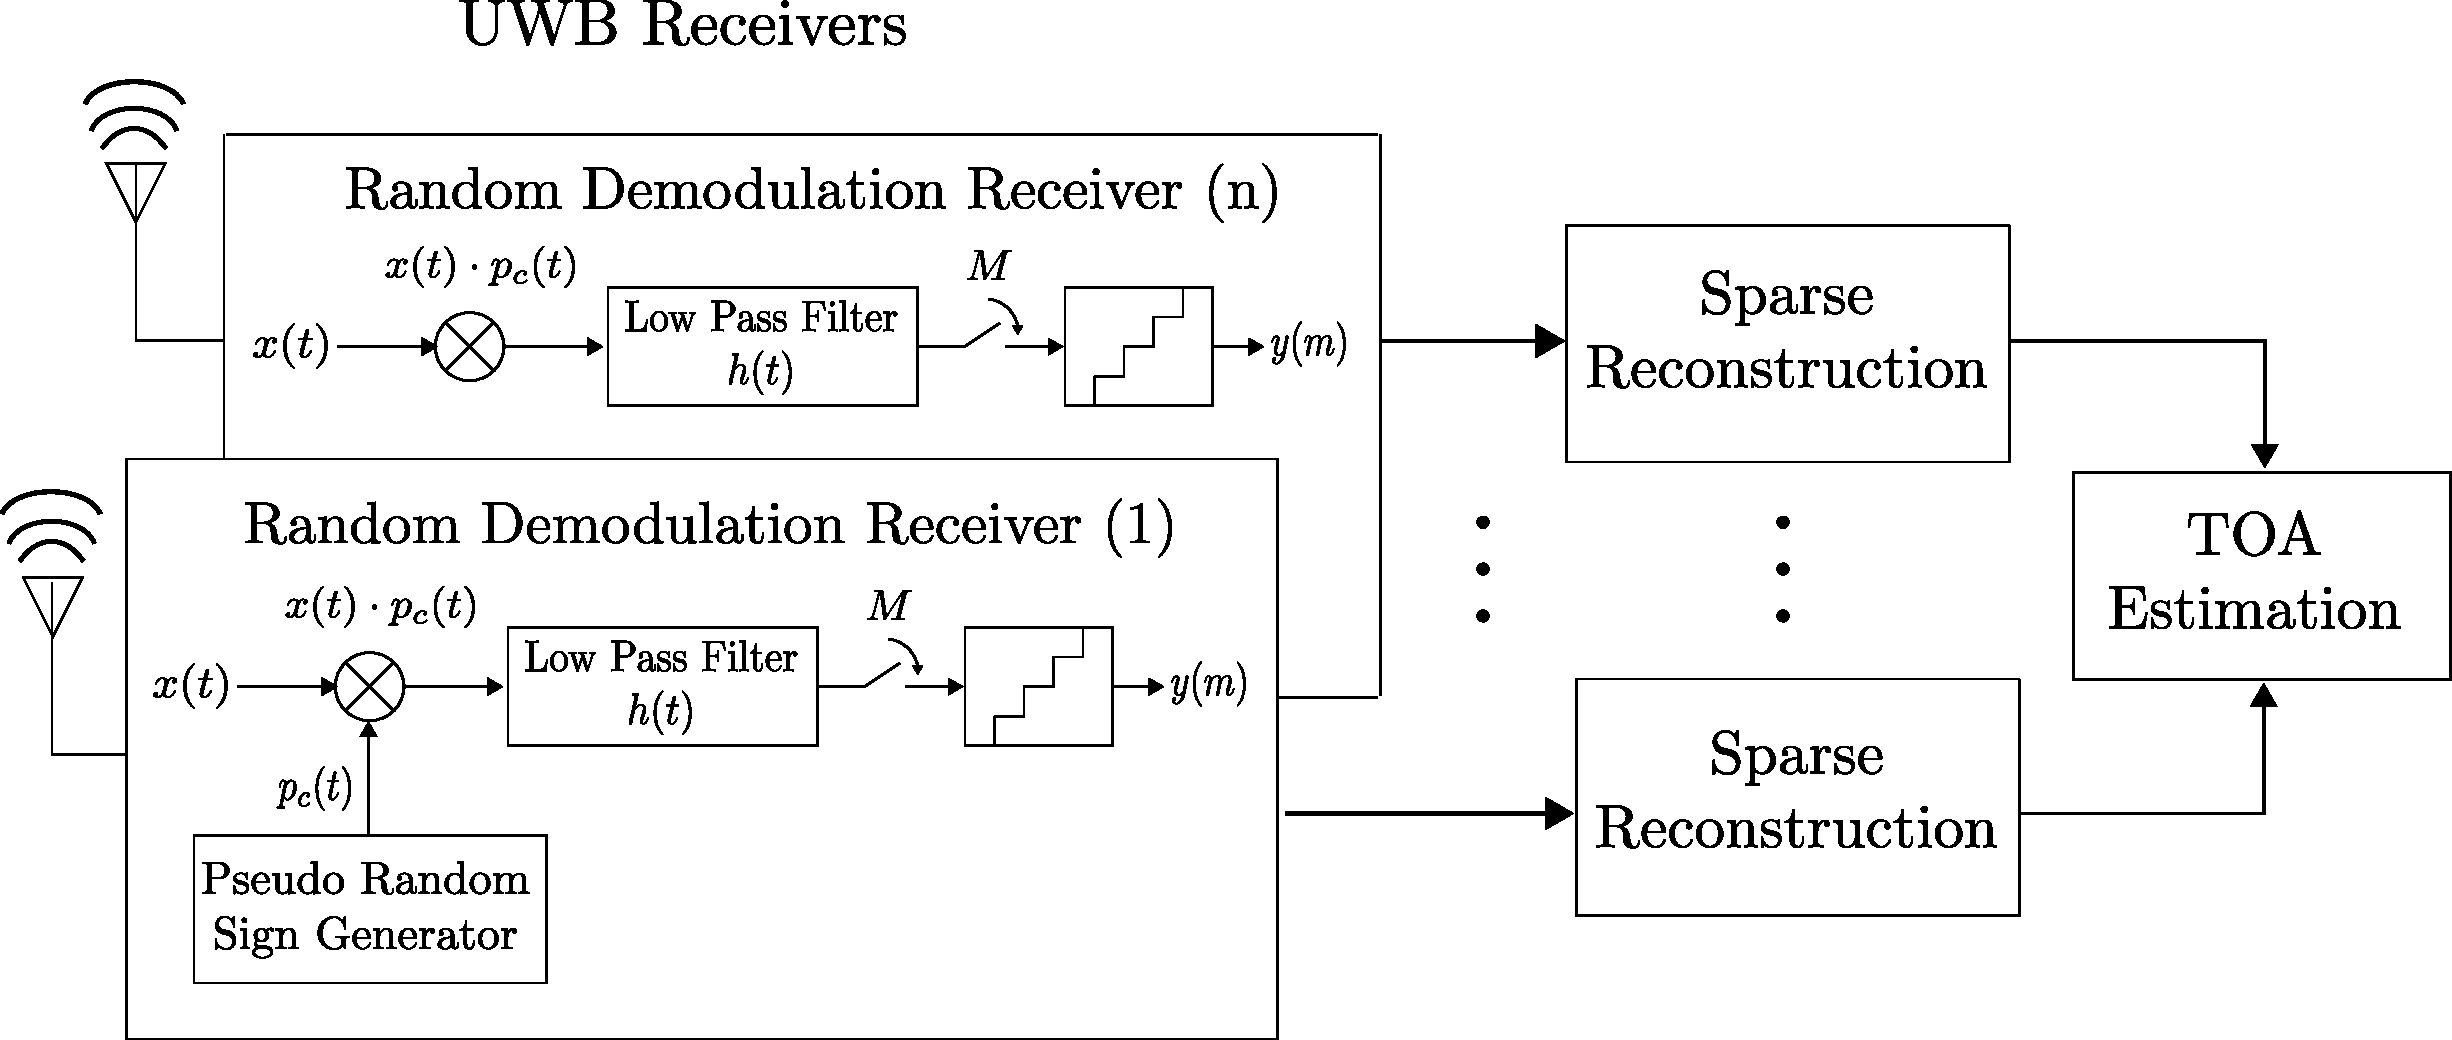
\includegraphics[width=0.5\columnwidth]{cs-uwb-design1.pdf}
\DeclareGraphicsExtensions.
\caption{Block diagram of compressive receiver implemented by random demodulator (RD). The components of RD includes a pseudo-random sign generator (PRSG), a low-pass filter (LPF), and a sub-Nyquist ADC}
\label{cs-uwb-design1}
\end{figure}

Typical recent researches embed the CS reconstruction algorithm at UWB receivers to improve the SNR of the received signal. As a result, it not only increases the performance of the positioning accuracy \cite{banitalebi2014compressive}, but also reduces the sampling rate to a relatively low level compared to the Nyquist rate. Among these compressive receivers, most of them develop the random demodulator (RD) \cite{kirolos2006analog} as the main structure of CS based UWB receivers \cite{yang2011compressive}. 

In this system, each compressive receiver realises the RD architecture that composed of a pseudo-random sign generator (PRSG), a low pass filter (LPF), and a sub-Nyquist rate analog-to-digital converter (ADC), shown in Fig.\ref{cs-uwb-design1}. 

Then the transmitted UWB signals are collected by group of low-rate distributed ADCs only using a minimal sampling rate of $1.7K(log(N/K))$ \cite{kirolos2006analog}, where $N$ stands for Nyquist rate and $K$ is the sparsity in transmitted UWB signals. Results in \cite{yang2013compressive} demonstrates that the new system successfully improves positioning accuracy. 

\subsection{Compressive Transmitters}
\indent \indent On the other hand, some researches embed the CS technique at the UWB transmitter and regarded it as a better solution than compressive receivers in terms of  system hardware power efficiency. The new architecture contains a random tap FIR at the transmitter, which accomplishes the CS random projection before UWB signals are transmitted \cite{zhang2009compressed}. Followed by distributed sub-Nyquist rate ADCs, the down-sampled signals are collected for TOA based algorithm. Simulation result \cite{zhang2009compressed} shows that the new compressive transmitter is suitable for detecting the indoor channel model with higher accuracy than traditional TOA based method. This architecture is also suitable for indoor positioning because the transmitted signal pulse and channel model keep the same. Besides, it meanwhile saves more energy cost since it contains less hardware mixers than compressive receiver based UWB system. However, the complexity of implementation a high data rate random tap FIR filters brings additional cost and becomes a main difficulty in applications.

\section{Energy Aware Random Mixing Transmitters}
\begin{figure*}[!t]
\centering
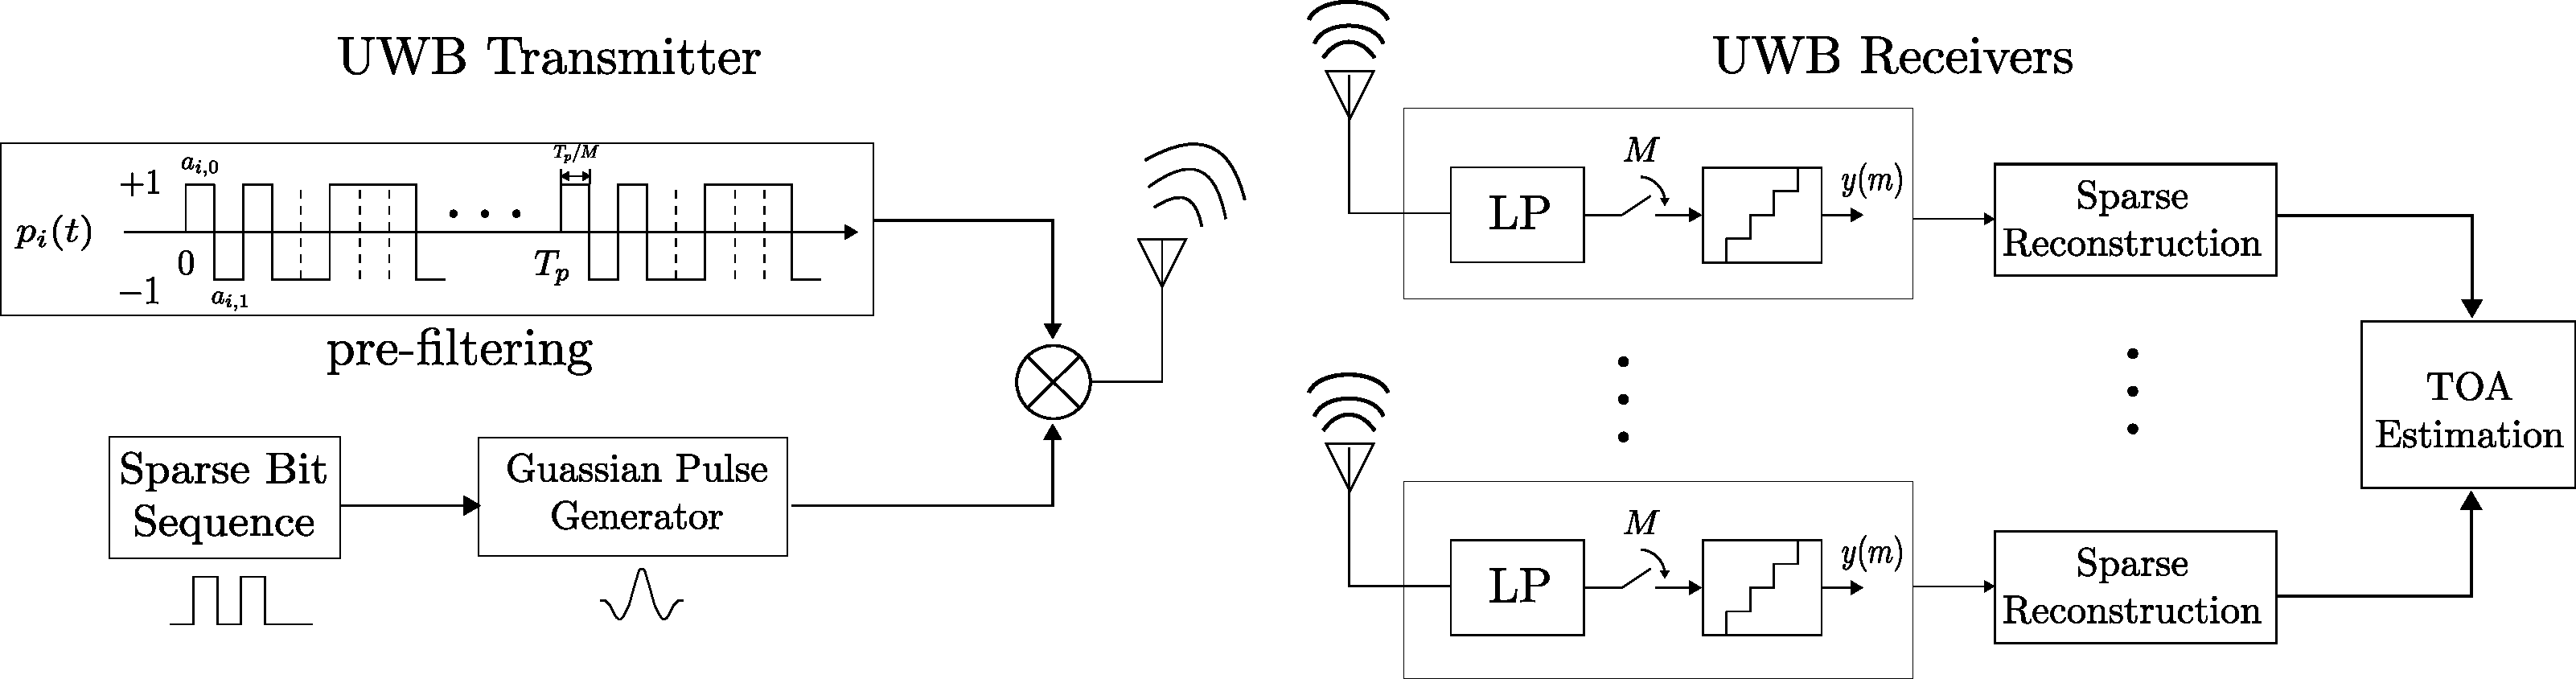
\includegraphics[width=0.85\columnwidth]{cs-uwb-design2.pdf}
\DeclareGraphicsExtensions.
\caption{Block diagram of low-rate compressive random mixing UWB positioning system.}
\label{cs-uwb-design2}
\end{figure*}

As mentioned, both compressive receivers and compressive transmitters suffer from high-data rate random projection operation, where the alternative rate of pseudo-random sequence is required (often equal or above 5 GHz in such cases). This requirement generates a heavy burden on bandwidth of hardware mixers and high frequency noise. 

In order to solve this problem but meanwhile preserve the energy efficient feature in compressive transmitters, this paper propose an low-rate compressive random mixing (CRM) UWB positioning system shown in Fig.\ref{cs-uwb-design2}: At the transmitter side, the new system provides a relatively low-rate pseudo-random sequence to mix the generated Gaussian pulses. At the receivers side, it sacrifices the compression ratio (or sampling rate) to catch up with the equivalent performance as that in the compressive receivers based UWB system. As a result, the trade-off between the random projection rate and the sub-Nyquist sampling rate offers a more energetic balanced system, where no hardware devices suffers from the limitation brought from the high data rate sequence. In addition, the positioning accuracy is successfully improved compared to the original UWB system. 

\paragraph{System Model}
Based on the IR-UWB indoor positioning system model in (\ref{eq_recv}), the new structure of our system can be regarded as shown in Fig.\ref{cs-uwb-design2}. At the transmitter, the a pseudo-random sequence (PRS) whose variables are chosen from ${-1,+1}$ are generated using a relatively low sub-Nyquist alternative rate. When a UWB pulse generated, first it will be randomly mixed by the pseudo-random sequence, and then broadcasted to indoor environment from the transmitter. Afterwards, receivers directly down-sample the signals at a relatively low rate. Finally, after processing the sparse reconstruction (i.e OMP or BP), the original TOA based algorithm can work for indoor positioning. In addition, these steps at receivers can be executed pipelined as \cite{yang2011compressive}. Hence, based on the workflow of the new architecture, the math model of this system can be represented as following matrix form (\ref{eq_sys_m}):
\begin{equation}
\label{eq_sys_m}
y = D * H * P * x
\end{equation}
where $y$ are discrete sampled observations from low rate ADCs at receivers, and $x$ is the generated UWB Gaussian pulses at traditional transmitters. Here $H$ is the correspondingly Toeplitz matrix which presents the signal convolution using IEEE 802.15.4a model in (\ref{eq_chan}), and $F$ stands for the random projection step, which is a diagnose matrix whose variables are randomly chosen from $\{-1,+1\}$ but alternatives at a sub-Nyquist low rate. The $D$ represents the downsampling behaviour. It is a $m\times N$ matrix ($m << N$) with 0-1 entries , and each of its rows contains a block of $\frac{m}/{N}$ contiguous ones, which has been used for simulation in \cite{tropp2010beyond}. Then $\hat x$ can be reconstructed from various sparse reconstruction algorithm such as BP, OMP and CoSaMP. At last, the recovered signal $\hat x$ is applied for TOA based positioning estimation.

\section{Simulation Results}
\indent \indent This experiment uses Matlab to evaluate the performance of the proposed system. In the simulation, the UWB waveform is a periodic simple pulse which is shaped by the second derivative Gaussian wave with a pulse duration of 1ns. The bandwidth of this signal is 8GHz. The UWB channel model is based on the IEEE 802.15.4a CM1 model for line of sight (LOS) indoor environment, and zero-mean additive white Gaussian noise (AWGN) is added to generate an average SNR of 10dB. The simulation results cover random points in an area of 10m $\times$ 10m $\times$ 10m space.

CS Basis pursuit denoising (BPDN) algorithm is used at the receiver to perform the reconstruction process. Figure 4 shows the results of the reconstruction successful rate against the receiver’s sampling rates. Existing RD based system achieves $100\%$ successful reconstruction starting at 200MHz sampling rate, but requires 10GHz PN sequence at each receiver. Our proposed system use much lower rate PN sequence (1GHz or 500MHz) at the transmitter and achieve $100\%$ successful reconstruction at 350MHz and 500MHz sampling rate. Hence, accuracy of the lower rate PN sequence system can be improved by using higher sampling rate at the receiver. Therefore, the simulation result shows that the proposed system can apply trade-off among random projection rate, sub-Nyquist sampling rate and reconstruction rate. This design significantly reduce the peak frequency (Nyquist rate in mixing waveform or receiving end) in the system with acceptable rate increase in receivers' ADC sampling rate. 

Table I compares the accuracy of the two CS based systems against conventional UWB based system which uses hypothetical 10GHz Nyquist sampling rate. Both CS based systems produces much lower errors then the conventional UWB based system, while the proposed RP system has similar performance as the RD based system. 

\begin{figure}[!t]
\centering
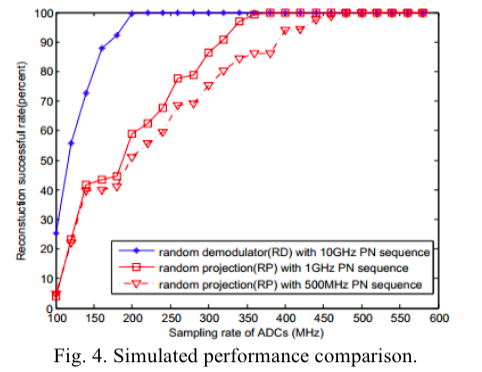
\includegraphics[width=0.5\columnwidth]{figs/res-pub.png}
\DeclareGraphicsExtensions.
%\caption{CS based TOA estimation average error under different compression ratio based on the IEEE 802.15.4a CM1 model for line of sight (LOS) indoor environment}
\label{res-pub}
\end{figure}
\begin{figure}[!t]
\centering
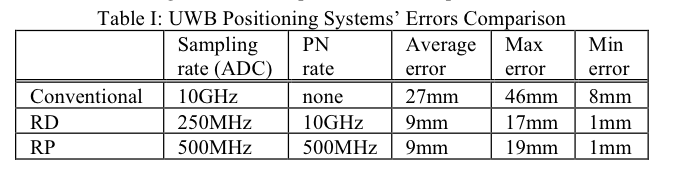
\includegraphics[width=0.75\columnwidth]{figs/res-pub-table.png}
\DeclareGraphicsExtensions.
%\caption{CS based TOA estimation average error under different compression ratio based on the IEEE 802.15.4a CM1 model for line of sight (LOS) indoor environment}
\label{res-temp}
\end{figure}

\section{Conclusion}\label{sct:cs_uwb_conclusion}
\indent \indent The compressed sensing is proven effective to improve the accuracy of IR-UWB positioning. However, most of papers do not concern the design complexity and energy cost in their implementations, for instance, the random mixing waveform is of extremely high frequency (in GHz). Our proposed compressive UWB positioning present a novel view of energy trade-off design, which is implemented by a low-rate random-projection at transmitters and low rate ADCs at receivers. This design significantly reduce the peak frequency (Nyquist rate in mixing waveform or receiving end) in the system with acceptable rate increase in receivers' ADC sampling rate. 

In this paper, following the architecture of waveform-based pre-coding at the transmitter\cite{zhang2009compressed}, we proposed a new compressive random mixing transmitters for UWB positioning. The main purpose of this system is to slow down the high rate mixing operation when building CS framework at transmitters. Simulation results demonstrate that our proposed CS-based UWB positioning scheme successfully decreases the high rate mixing operation by sacrificing a slight compression ratio ($<$ 10\%) or small increase on average error ($<$ 1mm). The new CS-UWB TOA positioning system can achieve a much higher positioning accuracy than the traditional system in mm level. Future research will focus on how to reduce the reconstruction running time so that the real-time performance can be enhanced. This aim relates to the compressive signal processing that will be mentioned in the next chapter.

%----------------------------------------------
%\section{Challenges in Ultra-Wideband System}

%Impulse-radio ultra wideband (UWB) technology has attracted widely usage in communication and positioning application, because of its advantages of extreme wide transmission bandwidth, fine time resolution, low-power consumption, low fading margin in dense multipath environment. There are two primary challenges exist, which are (1) how to gather energy over the rich multipath components, and (2) how to sample extremely high rate signals\cite{zhang2009compressed}. 

%%Additionally, in 2002, the FCC issued a first report and order allowing the unlicensed use of UWB devices, overlaid with existing devices, subject to a power spectral mask in a 7.5 GHz swath of spectrum. This has generated wide interest in potential UWB applications, and led to a rapid increase in the number of companies and governmental agencies working in UWB.

%%Many investigated applications for UWB are designed to operate in indoor environments. Indoor UWB systems must contend with dense multipath channels, which are characterised by tens or even hundreds of resolvable multipath components, and delay spreads typically orders of magnitude larger than the UWB pulse duration. Additionally, due to stringent FCC regulations, UWB systems are required to operate at a very low power emission level. These facts have led to several challenges pertaining to UWB transceiver design. Specifically, there are open challenges to be met in the areas of (a) UWB signal detection, (b) synchronisation, and (c) interference mitigation.

%%(1) Signal detection: Recent research has mainly concentrated on the Rake receiver and variants of the transmitted reference receiver as candidates for UWB detectors in dense multipath. However, both receivers have severe performance limitations. Specifically, the energy capture of the Rake receiver is relatively low for a moderate number of fingers, making its implementation impractical for UWB systems. Transmitted reference receivers suffer from a “noise-cross-noise” term, caused by the use of a noisy signal as a correlation or matched filter template. Consequently, a prohibitively large number of pilot symbols are required to overcome this limitation.

%Time reversal [5] provides a promising solution to the first problem [6]. In particular, the concept of time reversal has recently demonstrated in a real-time hardware test-bed [7], [8]. At the heart of time reversal, the channel itself is exploited as a part of the transceiver. This idea makes sense since the channel is time-invariant and reciprocal [9]. In principle, most of the processing at the receiver can be moved to the transmitter where energy consumption and computation are sufficient for many advanced algorithms. This framework is called waveform-oriented pre-coding.

%For instance, ultra-wide band (UWB) positioning always suffers from extremely high-rate signal detection. The compressive sensing (CS), which is considered as the optimal solution of acquisition and reconstruction for sparse signals, provides an alternative solution by implementing random projection at transmitters or receivers. However, these CS based UWB positioning systems still cannot avoid high-rate mixing operation when generating the PN sequence during random projection. 

%In this paper, we propose a new CS based UWB positioning system to solve this problem, which implements a relatively low-rate random pre-mixing at the transmitter and correspondingly sub-Nyquist rate sampling at receivers. As a result, the new system successfully eliminates the extremely high Nyquist rate in the system by sacrifices a small degree of compression ratio. Simulation results demonstrate the new system maintains outstanding performance in terms of positioning accuracy. 


%----UWB short introduction----

%\indent \indent Ultra-wide band (UWB) communication is widely used in wireless communication and associated with features as extreme wide transmission bandwidth, low-power consumption, shared spectrum resources in wide ranges etc. Among all applicable areas, UWB based accurate positioning and tracking in short range communication become popular since it provide resilient to multipath fading in hostile environment and outstanding robustness even in low signal-to-noise (SNR) situations \cite{cassioli2002ultra}. In addition, the requirements of high data rate and limitations of battery supply lead the impulse-radio ultra-wide band (IR-UWB) to become a suitable communication technique in short range high data rate communication. 

%However, along with the ultra high frequency transmission in IR-UWB communication, the receiving-end are suffering high sampling rate difficulty on its ADCs. Although many filter-bank based downsampling technologies are used to convert the high frequency into low frequency of original signal, complexity of multiple analog filters increase the design cost for hardware implementations.   

%Recently the CS framework is introduced to solve this problem for UWB, which provide a more convenient way to reduce the sampling rate at receivers. Comparing to traditional methods, the CS-based UWB omits the multiple analog filters and thus reduce the design complexity and cost. Simulation results demonstrate that the CS-UWB positioning can achieve high accuracy performance and providing energy-efficient design. 

%Our proposed work for UWB positioning system follows this idea, and additionally, we consider a further energy optimisation from aspect of architecture. While the formal CS-UWB uses Nyquist rate chipping sequence (or PN sequence) to fulfil random sampling behaviour for CS framework, however, this procedure forces Nyquist sequence and thus the high frequency does NOT omitted although sampling rate has been reduced. Our design aims at this problem, analyses a tradeoff between the rate of PN sequence and the sampling rate, and finally eliminates the Nyquist rate in entire system.  


%----performance describe in orignial latex---
%As shown in Fig.\ref{res1}, when the Sampling rate comes close to ???, the average error of all CS-based UWB system has been converges to less than 10mm. However, when the compression ratio continuously increases, the error converging speed of CRM-UWB cannot catch up with the speed of others. This is because that if we manage to reduce the highest rate at transmitters in CRM-UWB, as a result, the required sampling rate must be increased as a sacrifice at receivers, otherwise the estimation error rate will increase. Furthermore, if we increase the sub-Nyquist sampling rate  by 10\% of CR at receivers, which creates a revised system named CRM-UWB-R, then it produce outstanding performance: when compression ratio becomes less than 0.15 and continuously decreases, the advantage of the proposed CRM-UWB emerges: the error increasing speed is far slower than the others. This result suggests that the CRM-UWB-R (the revised low-rate compressive random mixing system) outperforms the traditional CS UWB positioning systems in terms of estimation error at lower compression ratio. 

%Besides, the CR-UWB, CPCT-UWB, and CRM-UWB all provide sub-mm estimation error with enough CS observations (CR $>$ 0.15), while the original UWB TOA system contains an average error around 3.92mm. Thus, CS UWB TOA positioning system can achieve a much higher positioning accuracy than the traditional system. 

%The Fig.\ref{res1} demonstrates the TOA estimation average error under different sampling rates. The received signal can be recovered from a certain amount of CS measurements $M$ which is far less than $N$ (Nyquist rate), where compression ratio (CR) equals $\lfloor{M/N}$. In the simulation, three types of different UWB positioning system are tested: 1) compressive receivers for UWB positioning (CR-UWB), where random demodulator is implemented at receivers, and the CR refers to the sampling rate of its ADC. 2) The CS pre-coding transmitter (CPCT-UWB), where Nyquist rate random projection is implemented at transmitters and downsampling is realised at its receivers. The CR refers to the downsampling rate at its receivers. 3) The proposed new architecture, low-rate compressive random mixing for UWB positioning system (CRM-UWB), where sub-Nyquist rate random projection is implemented at transmitters and downsampling is realised at its receivers. In this new system, CR refers to the downsampling rate at its receivers, and especially, the low-rate pre-filtering is accomplished by mixing a pseudo-random sequence (PRS) which alternates at a (CR + 10\%) of Nyquist rate. 

\chapter{Wideband Cognitive Spectrum Sensing}\label{C:wideband_css}

Cognitive Radio (CR) has been attracting many attention in recent researches with respect to the potential better utilisation performance of limited spectrum resources. In this chapter, we first propose an overview of cognitive radio networks. Then we focus on the bottleneck in its front-end sampling devices and investigate the typical CS framework for spectrum sensing in CR. 

\section{Introduction}

As the wireless techniques keep fast developing, the limited spectrum resource seriously restricts the fast increasing demand for more accessible bandwidth. As a result, the dynamic spectrum access (DSA) becomes necessary and popular, which enables unused spectrum accessed opportunistically, shown in figure \ref{dsa-cr-intro}.(a). 

Following this idea, the cognitive radio (CR) develops aiming at optimizing utilisation of idle bands for communications, without doing harm to the primary users (licensed spectrum) \cite{akyildiz2006next}. Correspondingly, the CR devices have to sense the environment (including spectrum usage, noise level etc) quickly and accurately, and reconfigure themselves to adapt the varying circumstance.

\begin{figure}
\centering
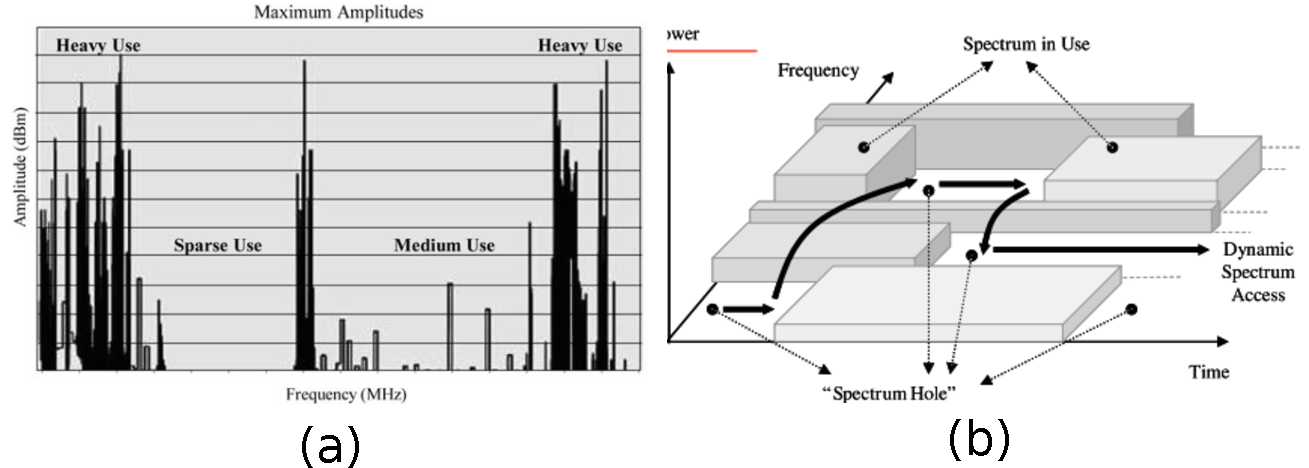
\includegraphics[width=0.85\columnwidth]{figs/cr-intro.pdf}
\caption{(a) The existence of unused spectrum resources; (b) The concept of spectrum holes}
\label{dsa-cr-intro}
\end{figure}

Therefore, in cognitive radios, the first and important procedure is to sense the unused bandwidth, termed as the spectrum holes and shown in figure \ref{dsa-cr-intro}.(b). If the band is detected as unused, the CR networks will use it for further communication. Otherwise, the CR moves to find other spectrum holes, or stays in the same band but avoid interference by changing its transmission power or modulation model.

However, trends of communicating requires higher frequency and wider bandwidth. As a result, signal acquisition significant is crucial according to the Nyquist sampling theory. What's worse, since CR should not generates additional interference to the licensed users, CR must limits its working power to a relatively low level (if CR do not change its modulation model). The demand for sensing with low power contradicts with the requirement for sensing in high sensitivity. Thus this contradiction makes the signal acquisition much more difficult. 

In conclusion, spectrum sensing becomes one of the most crucial problem for cognitive radios, and it is still an open issue. Then, compressed sensing will be introduced to be embedded into traditional spectrum sensing algorithms, in order to solve the problem and enhance the overall performance.

\section{Spectrum Sensing}\label{sct:ssm}

%re-wr:
A cognitive radio supports the capability to select the best available channel \cite{akyildiz2006next}, and the main functions for cognitive radios in xG networks can be summarized as \cite{haykin2005cognitive}, where the spectrum sensing to decide whether a particular sub-band of the spectrum is available or not, without harmful interference with primary users. It is the first procedure in cognitive radio networks where various parameters are detected for further spectrum management, spectrum mobility and spectrum sharing. 

%\begin{itemize}
%\item{Spectrum sensing:} detecting unused spectrum without harmful interference to primary users.
%\item{Spectrum management:} capturing the best available spectrum to meet user communication requirements.
%\item{Spectrum mobility:} maintaining seamless communication requirements during the transition to better spectrum.
%\item{Spectrum sharing:} providing the fair spectrum scheduling method among second users.
%\end{itemize}

\subsection{Aim: Spectrum Usage Detection}\label{sct:aim_ss}

According to the aim of spectrum sensing, the main task becomes to decide whether a particular sub-band of the spectrum is available or not, namely, to detect spectrum usage situation. A widely accepted idea is to detect the signal existence from licensed users' (primary users, PUs) communication at cognitive radio's receivers: if the PU's signal (in the particular sub-band) are not detected, cognitive radios can access the band for further communication; otherwise, CR cannot use the band. 

\subsection{Hypothesis Detection Model}

In this subsection, the problem of detecting the signal existence from PUs is modelled by two hypotheses in equation \ref{detect_hypo}: 
\begin{equation}
\label{detect_hypo}
\begin{aligned}
H0: y[n] = w[n]   \\
H1: y[n] = w[n] + x[n] 
\end{aligned}
\end{equation}
, where $x[n]$ is the primary user's signal, $y[n]$ is the vectorial observation, $w[n]$ is the noise, and $n$ refers to time slots. The hypothesis 1 suggests that the primary user's signal exists, while hypothesis 0 suggests no. Typically, the decision is made by comparing a predetermined threshold with test statistic $\Lambda(y)$ in equation \ref{detect_statistic}: 
\begin{equation}
\label{detect_statistic}
\Lambda(y) \mathop{\lessgtr}_{H_1}^{H_0} \alpha
\end{equation}
Then the performance of a detector is quantified by the receiver operating characteristics (ROC) curve, which presents the probability of detection $P_D = Prob(\Lambda(y) > \alpha, H1)$ and false alarm probability $P_fa = Prob(\Lambda(y) > \alpha, H0)$. 

\section{Traditional Detection Method}

\subsection{Narrowband Detection}

In this section, typical spectrum sensing approaches are introduced. Narrowband sensing algorithms can be suitably applied when the channel frequency response is flat. The following figure \ref{narr_spec_sens} demonstrates most typical architectures in narrowband spectrum sensing.

\begin{figure}
\centering
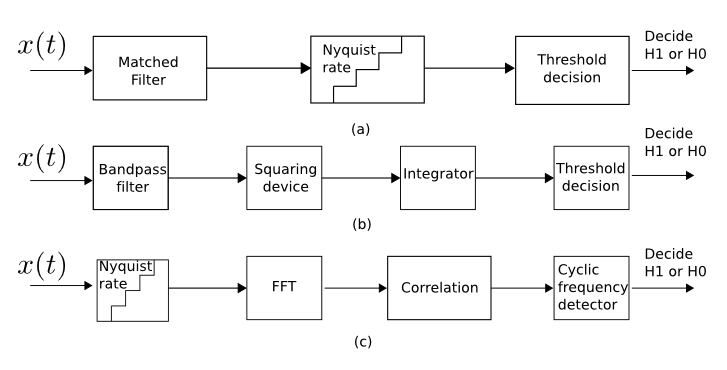
\includegraphics[width=0.75\columnwidth]{figs/narr_spec_sens.png}
\caption{Block diagrams for traditional narrowband detection architectures: $a)$ matched filtering detector; $b)$ energy detector; $c)$ feature detector}
\label{narr_spec_sens}
\end{figure}

\subsubsection{Matched filter}
In the figure \ref{narr_spec_sens}.(a), the matched filtering (MF) detector\cite{poor1994introduction} is presented. when the signal to be detected is perfectly known (i.e. mean and variance), the optimal test statistic is produced by matched filter by correlating the received signal to a template. However, the signal cannot always be known in practise, so sometimes it's not applicable. Besides, the carrier synchronisation is also a remained difficult problem.

\subsubsection{Energy detector}
In the figure \ref{narr_spec_sens}.(b), the energy detector (ED) \cite{urkowitz1967energy} is presented. In the case where the signal to be detected does not present structure template, the ED can produce the optimal test statistic by directly analysis the power and variance of the received signal. The implementation of ED is simple, but it suffers from poor detection results in low SNR environment. Besides, the ED cannot distinguish different primary signals at the same time.

\subsubsection{Feature detector}
In the figure \ref{narr_spec_sens}.(c), cycle-stationary feature detection (FD) \cite{enserink1994cyclostationary} is presented. If discrimination for primary signals and higher detection performance are required, the FD exploits the cyclic non-stationary features from primary signals. The cyclic features can be found in many typical modulated signals, for instance, in the orthogonal frequency-division multiplexing (OFDM) contains cyclic features in correlation structure due to the cyclic prefix (CP) between transmitted data. However, the computational cost is relatively high and long running time delay is always existing. 

\subsection{Nyquist Wideband Detection}\label{sct:wss}

In the scenarios where the bandwidth is sufficiently larger than coherence bandwidth of channel, wideband sensing is more suitable than narrowband sensing. For instance, it can be used for sensing the ultra-high-frequency (UHF) TV band, ranging from 300 MHz to 3 GHz, while the narrowband sensing providing single binary decision over whole spectrum is always not suitable for identifying individual spectrum access opportunities. The following figure \ref{nqys_spec_sens} demonstrates the typical architectures for wideband spectrum sensing and detection.

\begin{figure}
\centering
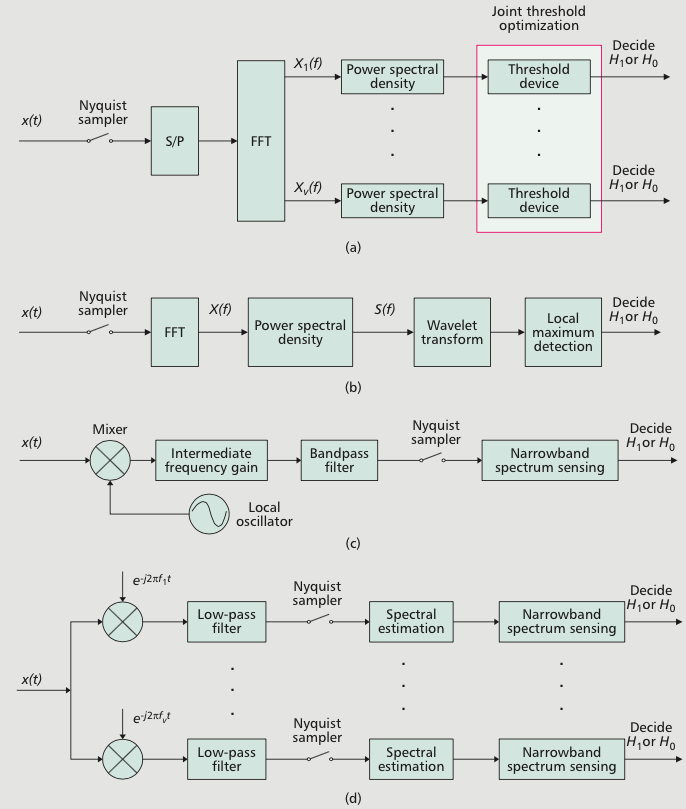
\includegraphics[width=0.75\columnwidth]{nqys_spec_sens.png}
\caption{Block diagrams for Nyquist wideband detectors architectures: $a)$ multiband joint detector; $b)$ wavelet detector; $c)$ sweep-tune detector; $d)$ filter-bank detector}
\label{nqys_spec_sens}
\end{figure} 

\subsubsection{Multiband joint detector}
In figure \ref{nqys_spec_sens}.(a), the multiband joint detector (MJD) \cite{quan2009optimal} is presented. The MJD first uses serial-to-parallel conversion (S/P) to divide samples into parallel data streams, then it process the FFT to divide spectrum X(f) into groups of narrowband spectrum. Then each binary hypothesis detection is performed and joint optimised at last. The high sampling rate and lower speed of joint optimisation is the main bottleneck.

\subsubsection{Wavelet detector}
In figure \ref{nqys_spec_sens}.(b), the wavelet detector\cite{tian2006wavelet} is introduced. The wavelet analysis of power spectral density (PSD) can provide significant border symbols of two neighbour sub-bands, the aim of detection becomes a spectral edge detection problem. However, the high sampling rate is also the bottleneck.

\subsubsection{Sweep-tune detector}
In figure \ref{nqys_spec_sens}.(c), the sweep-tune detector\cite{quan2009optimal, farhang2008filter} is displayed. This detector uses a special frequency mixing technique that 'sweep' across the frequency range of interest, to down-converts signals to a lower frequency. The adaptive local oscillator (LO) is used for 'sweep' procedure. However, the procedure of 'sweep' mixing generates too much time to wait.

\subsubsection{Filter-bank detector}
Also using the idea of down-conversion, the figure \ref{nqys_spec_sens}.(d) shows the structure of filter-bank detector \cite{farhang2008filter}. Not only following the technique which 'sweep' mixing the interest of signals, it also applies parallel structure to speed up the processing time by using filter-bank. As a result, the time cost of mixing reduces but the implementation cost largely increase.

\section{Sub-Nyquist Wideband Detection}

Different from Nyquist wideband detection, the sub-Nyquist spectrum sensing applies the multi-coset (MC) sampling, multi-rate (MR) sampling, or compressed sensing (CS) to reduce the required sampling rate. Before talking about CS based sampling, first we take brief look at MC and MR sampling.

\subsubsection{Multi-Coset Sampling}

The multi-coset (MC) sampling \cite{venkataramani2000perfect} applies blocks of parallel consecutive samples with special time offsets to sample, so that each channel has a task of low-rate sampling. Then joint spectrum recovery and further detection can be performed. The main difficulty is how to perform sampling channel synchronisation with highly accurate time offsets. The quality of the specific offsets is crucial for robustness in its spectral reconstruction.

\subsubsection{Multi-Rate Sampling}

The multi-rate (MR) sampling \cite{sun2013wideband} uses various sampling rates to wrap different sparse spectrum onto individual channels, and then use joint sparse spectrum recovery for further energy detection. Time synchronisation is no longer needed compared to the MC. But instead, the sacrifice is the hardware cost for parallel structure, as well as the increased sampling rate compared to original CS although the MR's sampling rate is still less than Nyquist rate. 

\section{CS based Detection Method}\label{sct:cwd}

\subsection{Introduction to Compressive Spectrum Sensing }\label{sct:css}

Cognitive spectrum sensing is another typical application suitable for compressed sensing. The applicability of Compressive spectrum sensing (CSS )mainly lies in two aspects:  

\paragraph{Sampling Rate}
The trend of higher frequency transmission is also suitable for cognitive radio, which leads to higher rate sampling rate at receivers. Thus it's reasonable to develop the CS based spectrum sensing techniques to reduce the sampling rate.

\paragraph{Flexibility and Energy}
The cognitive radio requires flexibility for sensing various  types of signals (TV signal, cell phone, satellites etc) in a relatively wide bandwidth. However, normal wideband spectrum detection uses filtering or mixing for down-conversion (then low-rate sampling). This approach require difficult analog implementations such as adaptive local oscillator(LO) for filter-banks(FB). Inversely, if the CS is used, then the system can get wider sensing (frequency) ranges without the hardware of LO or FB.

Therefore, the CS become popular in cognitive spectrum sensing. The figure \ref{comp_spec_sens} demonstrates the typical architectures in wideband spectrum sensing, and briefly analyse CS detectors. The similar CS based architecture can also be viewed in chapter \ref{C:compressed_sensing}.

\subsection{Compressive Detectors Overview}
\begin{figure}
\centering
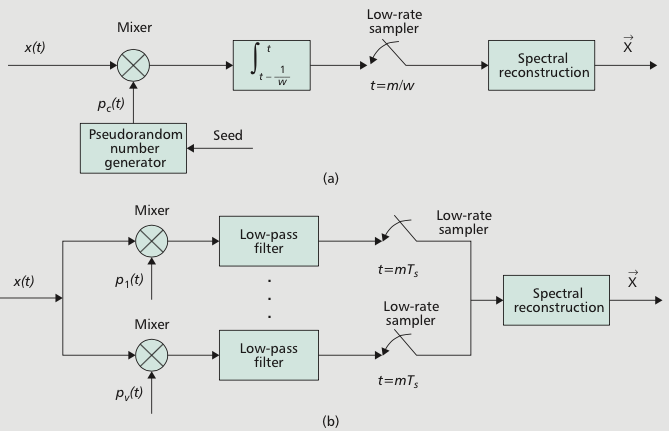
\includegraphics[width=0.75\columnwidth]{figs/comp_spec_sens.png}
\caption{Block diagrams for compressive wideband sensing architectures: $a)$ random demodulation based detector; $b)$ modulated wideband converter-based detector}
\label{comp_spec_sens}
\end{figure} 

\subsubsection{Demodulation based Detector}  
Figure \ref{comp_spec_sens}.(a) presents the random demodulation (RD) based detector\cite{tropp2010beyond}, which is an analog-to-information converter (AIC) for finite-length and discrete-time signals, and consists of pseudorandom wave generator, a mixer, and a low-rate ADC. The detailed architecture of RD is introduced in chapter \ref{C:compressed_sensing}. The reconstruction of RD sampled data involves $l1$-norm minimization (e.g. based BP, LASSO) or greedy method (e.g. OMP).
This design is simple, but easily affected by model mismatches and design imperfections.

\subsubsection{Modulated Wideband Converter based Detector}
Figure \ref{comp_spec_sens}.(b) displays the modulated wideband converter (MWC) based detector \cite{mishali2009expected} for the case where multichannel signals are designed to be detected. The MWC can be considered as a parallel structure of RD, and its architecture is introduced in chapter \ref{C:compressed_sensing}. The reconstruction of MWC involves the multiple measurement vector (MMV) sparse recovery which exploits the fact that the columns of original spectrum coefficients share the same sparsity pattern. Compared to the RD, MWC provides robustness against the noise and model mismatches.

\subsubsection{Cooperative Compressive Spectrum Sensing} 
%re-write{
Cooperative versions of spectrum sensing is an open issue, which aims at solving the hidden terminal problem \cite{akyildiz2006next} and improve sensing accuracy. The cooperative version of compressive wideband sensing have
 been developed \cite{tian2008compressed, wang2009distributed}. Here, individual radios can make a local decision about the presence or absence of a primary user, and these results can then be fused in a centralised or decentralised manner. However, a greater cooperation gain can be achieved by fusing all the compressed measurements, again in a centralised or decentralised manner. In general, such measurement fusion requires that each cognitive radio knows the channel state information (CSI) from all primary users to itself \cite{tian2008compressed}, which is cumbersome. But recent extensions show that measurement fusion can also be carried out without CSI knowledge \cite{fanzi2011distributed}.
%}

\subsection{An Instance: CS based Cognitive Radar System}
In \cite{stinco2014compressed} the CS is embedded to enhance the performance of cognitive radar that use wide operating frequency bandwidths for spectrum sensing and sharing. The compressive cognitive radar  utilises the typical CS techniques, including the random demodulation (RD) for signal acquiring, basis pursuit de-noising (BPDN) algorithm and discrete cosine basis (DCT) for sparse reconstruction, and classical energy detector (ED) for hypothesis analysis. 

\begin{figure}
\centering
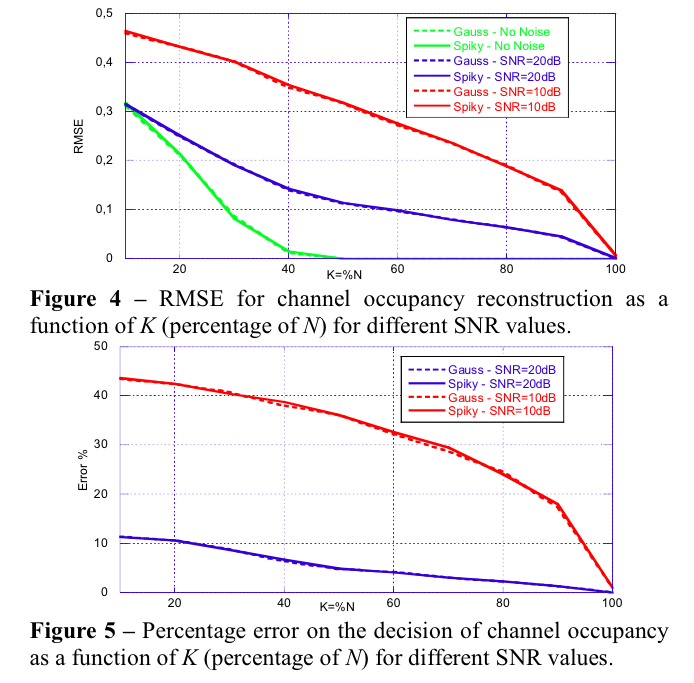
\includegraphics[width=0.75\columnwidth]{figs/cs-cogn-radar.png}
\caption{Block diagrams for mean square error and error detection performance of the proposed compressive cognitive radar systems}
\label{cs-cogn-radar}
\end{figure} 

The experimental results figure \ref{cs-cogn-radar} shows the CS based radar has appealing performance in low sampling rate (using only $ < 30\%$ of the total samples of the original signal) and low detection error in high SNR cases. But in low SNR environment, the proposed system still struggles and suffers. 

\newpage

\section{Further Sensing Task: Hybrid Signal Processing}

\begin{figure}
\centering
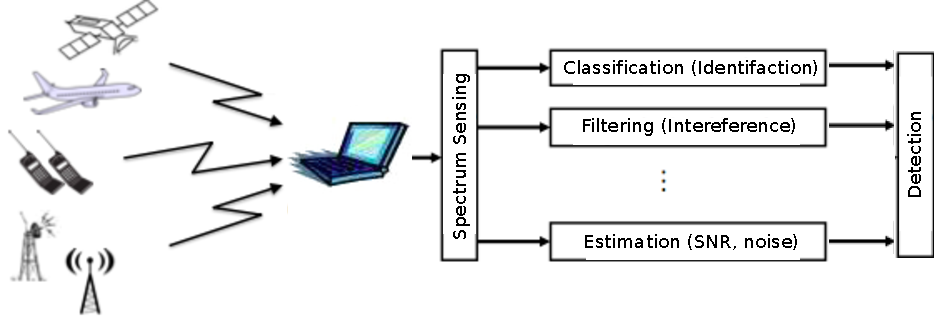
\includegraphics[width=0.75\columnwidth]{figs/hybrid_dsp.pdf}
\caption{Block diagram of hybrid signal sensing, processing and detection in cognitive spectrum sensing}
\label{hybrid_dsp}
\end{figure} 

According to the aim of spectrum sensing that we have talked in section \ref{sct:aim_ss}, the main task is to detect the signal existence of licensed users' (primary users, PUs) from cognitive radio's receivers.

Practically, in order to obtain high accurate detection result, a cognitive radio must keep monitoring almost every useful 'clues' to prove whether a spectrum band is used or not. Such clues (in physical layer) contains various information such as
signal to noise ratio (SNR), modulation mode, primary signal bandwidth, and primary signal power etc. 

As listed, there are too many informations to monitor at cognitive radios' receivers, so most of spectrum sensing algorithm only detect parts of the listed information, some detect power (energy detection), some detect partial signal (matched filtering detection), and others detect cyclic symbols (feature detection). 

As many of those method successfully accomplish the task in different scenarios, such as ED works well in high SNR cases, feature detection performs well in cases where primary signals contains strong periodic information, however, one of the key aims of designing a modern networks, is to make the network flexible enough, where hybrid types of primary signals communications (e.g. TV, mobile phone, radar) are mixed, and time-varying parameters (SNR, noise, power modulation type) based communications are allowed, shown as Figure \ref{hybrid_dsp}. This demand gives rise to a significant uncertainty in signals' appearance, and communication quality. As a result, in most practical cases, hybrid signal communication will co-exist, and for a higher detection results, pre-procedure such as filtering and classification for detection should be considered.

As a result, in cognitive radio, although detection is still a main task, but 
in order to efficiently detect co-existed primary signals, filtering (e.g. interference cancelling),  classification (e.g. hybrid signal separation), and estimation (e.g. SNR prediction) are also needed and regarded as useful auxiliary methods for further complex detection algorithms. 

Therefore, those assistant methods involves many traditional signal processing methods, and how to suitably apply them to process CS sampled data is a big deal because those data are non-linearly sample while traditional DSP algorithms are aiming at linear samples. In this sense, CS reconstruction are
needed, but it is time-consuming.

The problem shows us a further important issue for hybrid signal's processing in CS based cognitive radio, and more details will be introduced as our future research directions in chapter 6. 

\section{Challenges and Discussion}

The compressed sensing based wideband spectrum sensing for cognitive radio provide its outstanding feature in reducing the sampling rate. However, the corresponding drawbacks emerge in real-time ability and energy consumption, mainly due to its computational expensive non-linear reconstruction and energy consuming characters: 

\subsection{Long-Time Feedback Delay}
Accuarcy is cruical for primary detection. Hence, if we applies CS for sampling, the convex optimisation (e.g.basis pursuit) is always needed for data recovery since it provides better accuracy and robustness comparing to greedy methods (chapter \ref{C:compressed_sensing}). However, convex optimisation is time consuming, which cause too long time to fast feed-back. Since feed back is very important for CR, which is responsible to avoid interference and quick reconfiguration, agility and reconfigurablity may reduce.

\subsection{Mismatch for Traditional Signal Processing}
The reconstruction algorithms for CS is non-linear, which indicates that the recovered data are not directly suitable for conventional digital signal processing where traditional recovering only requires cardinal sinc interpolation (linear process). This brings difficulty in directly reuse the traditional method for sensed data.

\subsection{High Energy Cost}
The heavy reconstruction for CS not only brings large time-delay, but also additional energy cost. Compared to linear recovery in traditional approaches, the CS based signal detection additionally required the block for spectrum recovery before further hypothesis detection. 

\section{Conclusion}
Cognitive radio has been widely used and attracting many research attentions in its spectrum sensing techniques. In this chapter, traditional sensing approaches such as energy detection and feature detection are introduced. In order to solve the detection task for wideband and high frequency signals, compressed sensing based spectrum sensing (CS-CSS) is introduced and demonstrated. However, the compressively sampled data does not directly match the traditional processing algorithms.

Then here comes the question: what if we directly perform hypothesis detection without CS reconstruction? If the idea is achievable, the additional energy cost will be eliminated so that the entire energy reduces. Besides, not only detection, if we can expand this idea to filtering, estimation, then more intelligent-based scheme for cognitive radio can be supported in physical layer. The answer refers to our future research aims that shown in the next chapter.

%However, in cognitive radio, most of tasks for spectrum sensing are related to detection, estimation, filtering, classification. This contradiction leads the large additional loss in energy usage and time utilisation when we applies the CS to reduce the sampling limitation in wideband sensing for CR. Then noticing the fully reconstruction is always not needed, we will discuss the future direction in the next chapter, for directly processing compressively sampled data in CR, which aims at extracting effective information without fully recovery so that the entire real-time capability and energy efficiency will be significantly increased. 

%--------------------------------------------------------------------

%This is the common problem termed as cognitive spectrum sensing (CSS), that we face in modern signal processing systems, where the ADCs now use CS framework to solve the problem in high sampling rate. Similarly, CR devices recently apply the CS framework, and successfully achieves low-rate wideband signal acquisition while keeping the sensing accuracy in a high level. 

%--------------------------------------------------------------------
%re-write{
%A fundamental difference between CS and classical sampling is the manner in which the two frameworks deal with signal recovery, i.e., the problem of recovering the signal from the measurements. In the Shannon-Nyquist framework, signal recovery is achieved through sinc interpolation?a linear process that requires little computation and has a simple interpretation. In CS, however, signal recovery is achieved using nonlinear and relatively expensive optimisation-based or iterative algorithms [xx3?5]. Thus, up to this point, most of the CS literature has focused on improving the speed and accuracy of this process [xx6?9].

%However, signal recovery is not actually necessary in many signal processing applications. Very often we are only interested in solving an inference problem (extracting certain information from measurements) or in filtering out information that is not of interest before further processing. While one could always attempt to re- cover the full signal from the compressive measurements and then solve the inference or filtering problem using traditional DSP techniques, this approach is typically suboptimal in terms of both accuracy and efficiency. 

%Our future work takes some initial steps towards a general framework for what we call compressive signal processing (CSP), an alternative approach in which signal processing problems are solved directly in the compressive measurement domain **without** first resorting to a full-scale signal reconstruction.
%}

%--------------------------------------------------------------------
%\section{Cognitive Radio and Spectrum Sensing}\label{sct:cr_and_spectrum_sensing}

%Conventionally, licensed spectrum is allocated in long term and intended to be used only by primary users. However, as the increasing demand for higher data rates for communications, the limitation of the inefficiency usage of licensed spectral resources becomes a great bottleneck. Hence, the idea of opportunistically accessing the unused spectral resources (dynamic spectrum access, DSA) turns to be popular and motivates the develop of cognitive radio (CR). In other words, cognitive radio [2, 3] has become a promising solution to solve the spectrum scarcity problem. 

%For each cognitive radio network, the second users (SUs, unlicensed users) are able to reuse idle spectrum for communications without doing harm to the primary users (PUs, licensed users) when PUs are absent. Further more, cognitive radio can be considered as an developed software-defined radio (SDR) %[Wideband spectrum sensing for cognitive radio networks- a survey]that automatically senses its surrounding environment (e.g. noise level, spectrum usage ,RF stimuli etc) and intelligently adapts its configuration (i.e. operation parameters) to varying network infrastructure, in order to meet the quality of service.

%--------------------------------------------------------------------

%re-write [Wideband spectrum sensing for cognitive radio networks- a survey]
%Cognitive radio is an advanced software-defined radio that automatically detects its surrounding RF stimuli and intelligently adapts its operating parameters to network infrastructure while meeting user demands. Since cognitive radios are considered secondary users for using the licensed spectrum, a crucial requirement of cognitive radio networks is that they must efficiently exploit under-utilised spectrum (referred to as spectral opportunities) without causing harmful interference to the PUs. Furthermore, PUs have no obligation to share and change their operating parameters for sharing spectrum with cognitive radio networks. Hence, cognitive radios should be able to independently detect spectral opportunities without any assistance from PUs; this ability is called spectrum sensing, which is considered one of the most critical components in cognitive radio networks.

%------------

% \subsubsection{X-Digital Signal Processing}
% Recent representative applications for CS signal processing focus on establishing interfaces to link the CS recovered data to the traditional signal processing. One of the popular CS based signal processing architectures is the X-DSP in Xampling\cite{mishali2011xamplingsignal}. This architecture is designed for joint sparse support detection and filtering via the samples from the MWC. The multi-band signal can be presented in quadrature representation:
% \begin{equation}
% \label{eqn_xdsp}
% x(t) = \sum_{i=1}^{N/2} I_i(t) cos(2\pi f_it) + Q_i(t)sin(2\pi f_it)
% \end{equation} 
% , where $I_i (t)$ and $Q_i(t)$ are the real-valued narrow-band signals, and $f_i$ is the unknown carrier frequency. 
% In the former section of modulated wide-band converter, recovering the signal $x(t)$ via MWC is achieved by using the MMV based CS reconstruction. However, since the frequency of the carrier $f_i$ is still unknown, although $z[n]$ in (\ref{eqn_zn}) is recovered, it's not approximate for standard DSP algorithms.
% %The subspace algorithm needs to estimate $f_i$ , $I_i(t)$ and $Q_i(t)$.
% %it is insufficient since the fine recovery of the multi-band signal requires 
% %the information $I(t)$ and $Q(t)$ are not contained in the $z[n]$ in (xa), and the carrier frequency is unknown. Therefore, although z[n] is recovered it's not suitable for standard DSP algorithms.  
% In \cite{mishali2011xamplingsignal}, a refined support detection algorithm, Back-DSP, is proposed by assuming zero cross-correlation between $I_i(t)$ and $Qi(t)$. The Back-DSP algorithm consists of the following steps: %reviseBegin
% 
% 1. Refining the coarse support estimate $f_i$ to the actual band edges using prior information of the minimal width of a single band and the smallest spacing between bands.
% 2. Obtain a sequence $s_i[n]$ for each $1 ≤ i ≤ N/2$, such that $s_i[n]$ contains the entire contribution of exactly one band.
% 3. Estimating $f_i$ using a digital version of the balanced quadricorrelator(BQ) from $s_i[n]$. The information signals $I_i(t)$ and $Q_i(t)$ are obtained based on $f_i$.
% 
% With Back-DSP, we can now reconstruct x(t) using \ref{eqn_xdsp}, which requires only N mixers, filters and DACs. In addition, note that once the information signals $I_i(t)$, $Q_i(t)$ are obtained, error correction DSP algorithms can be employed to improve the overall robustness to noise. %reviseEnd

% %------------------------------------------------------
% 
% \subsection{Hypothesis Test}
% 
% The aim of spectrum sensing is to decide whether a particular sub-band of the spectrum is available or not. In other words, the procedure is to discriminate based on two hypotheses in equation \ref{detect_hypo}: 
% \begin{equation}
% \label{detect_hypo}
% \begin{aligned}
% Hypothesis0 (H0): y[n] = w[n], \quad n = 1,..., N   \\
% Hypothesis1 (H1): y[n] = w[n] + x[n] , \quad n = 1,..., N
% \end{aligned}
% \end{equation}
% , where $x[n]$ is the primary user's signal, $y[n]$ is the vectorial observation, $w[n]$ is the noise, and $n$ refers to time slots. The hypothesis 1 suggests that the primary user's signal exists, while hypothesis 0 suggests no. Typically, the decision is made by comparing a predetermined threshold with test statistic $\Lambda(y)$ in equation \ref{detect_hypo}: 
% \begin{equation}
% \label{detect_hypo}
% \Lambda(y) \mathop{\lessgtr}_{H_1}^{H_0} \alpha
% \end{equation}
% Then the performance of a detector is quantified by the receiver operating characteristics (ROC) curve, which presents the probability of detection $P_D = Prob(\Lambda(y) > \alpha, H1)$ and false alarm probability $P_fa = Prob(\Lambda(y) > \alpha, H0)$. 
% 
% 
% %------------------------------------------------------
% 
% \begin{itemize}
%   \item \textbf{matched filtering \cite{poor1994introduction}} In the case where the signal $x$ to be detected is perfectly known (i.e. mean and variance), then the observation $y ~ N(x, \delta^2 I)$ under $H1$, and the optimal test statistic of the matched filter becomes: 
% \begin{equation}\label{match-filter}
% \Lambda(y) = Re[x^H y] \mathop{\lessgtr}_{H_0}^{H_1} \alpha
% \end{equation}  
% However, in practice the signal and noise parameters are not always known to the system, and its required carrier synchronization is difficult to implement. The hardware architect is shown in figure \ref{narr_spec_sens}.a.
%   \item \textbf{energy detection \cite{urkowitz1967energy}} 
% In many cases, the signal to be detected does not present enough structure information, then energy detector produces the optimal choice of detection by choosing the test statistic $\Lambda(y)$ as 
% \begin{equation}
% \Lambda(y) = \frac{y^2}{\delta} \mathop{\lessgtr}_{H_0}^{H_1} \alpha
% \end{equation}
% The implementation are of energy detector is simple shown in \ref{narr_spec_sens}.b. However, it cannot distinguish the different primary users signals, and provides poor detection performance in low SNR scenarios. 
%   \item \textbf{feature detection} cyclostationary feature detection \cite{enserink1994cyclostationary} detects and discriminate between different types of primary signals by exploiting their cyclic non-stationary features. For instance, the orthogonal frequency-division multiplexing (OFDM) signal have a explicit correlation structure due to the cyclic prefix (CP) between transmitted data at the transmitter. The architecture of this detector is presented in \ref{narr_spec_sens}.c. However, the computational cost is relatively high.
% \end{itemize}
% 

%----------------compressed sens vs filter-bank------------

%In such case, if weconvert the signals for lower rate sampling, the analog filter-bank must be very complex design with heavy cost, for instance, large filter bank which covers the whole bandwidth, or adaptive filter but cost long time frequency shifting. If we intend to reduce the design complexity and cost, however, the sampling rate should be relatively high with less filters for down-conversion. 

%----hypothesis model----
% The aim of spectrum sensing is to decide whether a particular sub-band of the spectrum is available or not. In other words, the procedure is to discriminate based on two hypotheses:
% \begin{equation}
% H0: y = w \quad (noise case)
% H1: y = w + x \quad (primary signal case)
% \end{equation}
% , where $x$ is the primary user's signal, $y$ is the vectorial observation, $w$ is the noise, and $n$ refers to time slots. Typically, the decision is made by comparing a predetermined threshold with test statistic $\Lambda(y)$ ideally defined by the likelihood ratio. The performance of a detector is quantified by the receiver operating characteristics (ROC) curve, which presents the probability of detection $P_D$ and false alarm probability $P_fa$. 
% \begin{equation}
% P_D = Prob(\Lambda(y) > \alpha, H1)
% P_fa = Prob(\Lambda(y) > \alpha, H0)
% \end{equation} 

\chapter{Future Work: Novel Signal Processing for CS Spectrum Sensing} 
\label{C:csp_css}

In the last chapter \ref{C:wideband_css}, we have discussed the main drawback in compressed sensing based spectrum sensing (CS-CSS) which derives from the computational non-linear CS reconstruction. As a fact, the CS framework sacrifices the time and energy performance in reconstruction produce (in return, the sampling rate is reduced). In order to solve this problem, this chapter focuses on exploring the potential approach of directly analysing compressive measurements without fully CS reconstruction. The new approach is termed as compressive signal processing (CSP), and it will be used for compressive spectrum sensing (CSS) in cognitive radio network (CRN), so that the drawback may be overcome in our proposed CSP based CSS systems. 

\section{Introduction to CSP}

The compressed sensing based wideband spectrum sensing for cognitive radio provides its outstanding feature in reducing the sampling rate. However, the corresponding drawbacks emerge in real-time ability and energy cost, mainly due to its computational complex non-linear reconstruction and energy cost in entire cognitive radio systems.  

However, many signal processing applications such as detection, classification, estimation and filtering do NOT require entire signal reconstruction \cite{davenport2010signal}. For instance, cognitive radios are aiming at processing the hypothesis detection rather than fully recovering the primary signals. In these cases, the aim of CS fully recovery is no longer necessary, so processing schemes like 'directly analysis without recovery' or 'partial recovery then analysis' become possible and applicable for cognitive spectrum sensing. 

This novel idea derives from the compressive signal processing (CSP)\cite{davenport2010signal}, which aims at extracting information directly from compressive samples without fully recovery.  

\subsection{Literature Review}

In \cite{ohlsson2013compressive}, the shift retrieval problem for compressive samples is researched. Rather than recovering CS data then analysing the shifted distance, the author develops efficient algorithms and proofs for directly recognising the shift distance from CS data. Valsesia et al \cite{valsesia2014compressive} develops the circulant sensing matrix based processing for compressive measurements, which displays an potential CSP application for convolution based models and is suitable for filtering or channel impulse response involved cases. Especially, for cognitive radio spectrum detection, a CSP based energy detector is designed in \cite{appaiah2013spectrum}. Further, Guo et al develops CSP for feature detector in \cite{guo2013feature} and pattern clustering is achieved.

\subsection{Proposed Research}

Since so far the CSP concept is always only defined in the theory level and has not been widely applied to CSS field, we believe there still exists many worthy research area and cases for CSP based spectrum sensing. In other words, CSP based cognitive spectrum sensing is still a relative new approach which applies the CS but throw away some CS drawbacks for CR spectrum sensing. 

\section{Potential CSP Applications In Spectrum Sensing}

The following sections are organised as different function introduction for CSP based cognitive radio spectrum sensing, including filtering, detection, estimation. Some related potential application for CS-UWB and CS demodulation are also introduced.

\subsection{CSP based Filtering}\label{sct:csp_filter}

In scenarios where cognitive spectrum sensing requires filters, the design cost for analog filters are expensive. Here we may use CSP based filtering to transform the analog filter to digital filter, which omits the implementation of hardware design for filters.

\subsubsection{Filter Domain Transform}

Assume that the filter's impulse response is $h$ (with length of $N_h$) and its corresponding matrix form is $H$, then $H$ is a circulant sensing matrix. 

Then, according to a CSP related theory in \cite{valsesia2014compressive}, it possible to exchange the $H$ and $\Phi$ (compressed sensing matrix), sometimes in CS frameworks, the effect of analog filter equals the effect processed by digital filters. The compressive measurements $y$ can be directly processed by filtering $H$ without recovery in some cases \ref{csp-filter} as follows:  
\begin{equation}
\label{csp-filter}
\hat y = \Phi H x = H \Phi x = H y \quad, where \quad i \in [1,m-N_h+1].
\end{equation}
, where the $\Phi$ is compressed sensing matrix with size of $m \times N$.  Consequently, by moving the filtering from analog to digital part, large amount of hardware complexity could be omitted. 

\begin{figure}[!t]
\centering
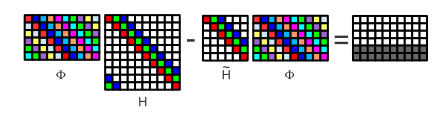
\includegraphics[width=0.75\columnwidth]{figs/csp-filter-thm.png}
\DeclareGraphicsExtensions.
\caption{Block diagram of exchanging order of circulant matrix. $H$ is corresponding impulse response of filter, $\Phi$ is the compressed sensing matrix. The exchanging sacrifice is the loss of rows in the results (matrix in the right side of equal sign).}\label{csp-filter-thm}
\end{figure}

\subsubsection{Interference filtering}

In cases where useless information is redundancy for further recovery in CS framework, or specifically where some sub-bands are priorly known in the compressive cognitive spectrum sensing, system using CSP can regard those useless information as interference, which applies CSP to achieve the procedure of 'sample-then-filter' to compressive data rather than sample-recover-then-filter it. 

Assume a sparse signal $x \in R^N$ which consists of two components:
\begin{equation}
\label{csp1}
x = x_s + x_I, \quad x_S \in S_S\; and\; x_I \in S_I
\end{equation}
, where the $x_S$ contains the spectrum of interest and the $x_I$ stands for the useless information. After the CS acquisition, we gain $y = \Phi x = \Phi(x_S + x_I)$. Then our aim is to wipe out the contribution of $\Phi x_I$ from the observation $y$ before recovering $x$. The following theorem provide the applicability of this idea:  
\begin{theorem}\cite{davenport2010signal}
\label{csp2}
Suppose that $\Phi$ satisfies the $\delta$-stable RIP for all $x_S\in\Sigma_S$ and $x_I\in\Sigma_I$, where $I$ is a $K_I$ dimensional subspace of $R^{N}$. Assume that $\Psi_I$ is an matrix whose columns constructs an orthogonal basis for the $K_I$ dimensional subspace. Define the matrix $P_{\Omega} = \Phi\Psi_I(\Phi\Psi_I)^{\dagger}$ and $P_{\Omega^{\perp}} = I-P_{\Omega}$. For any $x \in \Sigma_S \cup \Sigma_I$, we regard $x = x_S + x_I$, where $x_S \in s_S$ and $x_I \in s_I$, then
\begin{equation}
\label{csp3}
P_{\Omega^{\perp}} \Phi x = P_{\Omega^{\perp}} \Phi \hat x ,\quad
\frac{\delta}{1-\delta} \leq \|P_{\Omega^{\perp}} \Phi \hat x\|_2 \leq 1 + \delta 
\end{equation}
\end{theorem}
The theorem \ref{csp2} proofs that there exists a matrix $P_{\Omega^{\perp}}$ which is nearly orthogonal to the useless information $x_I$ such that $P_{\Omega^{\perp}} x_I \approx 0$. Hence the matrix $P_{\Omega^{\perp}}$ is the filter for selecting the desired signal $x_S$. we can apply this theory to construct a filtering matrix in CS acquisition model if the support of the $x_I$ is known. 

\subsection{CSP based Detection}\label{sct:csp_detect}
\begin{figure}[!t]
\centering
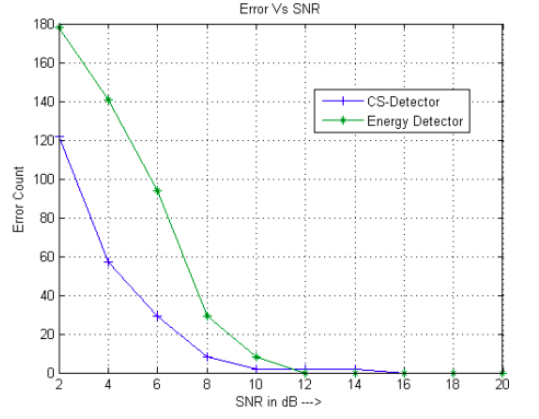
\includegraphics[width=0.5\columnwidth]{figs/csp-detec_vs_ED.png}
\DeclareGraphicsExtensions.
\caption{Block diagram of performance comparison between the CSP detector (compressive signal processing based detector) and ED (energy detector) from aspect of signal to noise ratio and detection error.}\label{csp-detec_vs_ED}
\end{figure}

\subsubsection{CSP based Energy Detector}
Davenport et al \cite{davenport2010signal} develops the theorem to directly build up hypothesis detection directly through compressed samples. Assume the detection is based on two hypotheses in 
\begin{equation}
\begin{aligned}
H0: y = \Phi w  \\
H1: y = \Phi (w + s)
\end{aligned}
\end{equation}
, where $s$ is the primary user's signal, $y$ is the vectorial observation, $\Phi$ is compressed sensing matrix (e.g. the random demodulation), and $w$ stands for the noise. Then the following equation \ref{csp-detect} presents the structure of CSP based detector. 
\begin{equation}
\label{csp-detect}
\Lambda(y) = (\Phi \Phi^T)^{-1} \Phi s \quad \mathop{\lessgtr}_{H_1}^{H_0} \quad \alpha
\end{equation}
In \cite{appaiah2013spectrum}, the experimental results of comparing CSP-detector and traditional energy detector (ED), is shown in figure \ref{csp-detec_vs_ED}. It has been shown that CS based Detector can provide better Error vs SNR performance. 

One defect of this simulation result is that, the paper does not discuss blind sensing techniques for cases where the information of primary signal $s$ is unknown to us. Thus further developing for CSP based blind sensing is a potential direction. 

\subsubsection{CSP based Cyclic Feature Detector}
%re-write:
Guo et al \cite{guo2013feature} develops CSP for feature detector in  and achieves pattern clustering.
The work generates the compressive spectrum measurement by utilizing both the cyclic-stationary feature and sparsity prior knowledge at the spectrum sensing front end. Then the paper applies the compressive CSP without the need of signal or feature reconstruction. 

However, as the author states that \cite{guo2013feature}, the CSP feature detection model is still simple. So how to analyze the spectrum pattern recognition performance in a more complicated CRN environment is open issue. For instance, with large-scale SUs and non-Poisson PU traffic models. Also, More efficient machine learning schemes (such as information geometry) can be used to recognize the PUs’ signal patterns after obtaining the CS samples via CSP scheme. 

\subsection{CSP based Estimation}\label{sct:csp_estim}

Since the signal-to-noise-ratio, sparsity order are crucial factors which seriously affects the performance of compressive detectors, CSP based estimation becomes popular for cognitive radio. 

This technique make CR be able to directly predict the level of sparsity or noise, so that CR can vary the sampling rate or change the detection algorithms based on those predicted information.

\subsubsection{Sparsity Order Estimation}

For instance, the sparsity order of the spectrum occupancy is time-varying in CR networks. If CR intends to fully exploit the CS framework, the sampling rate of CS receiver should keeping adjusting to sparsity orders. 

Therefore, estimating the sparsity orders in very important, and the \cite{sharma2014compressive} develops an approach which analysis sparsity order through asymptotic eigenvalue probability distribution function (aepdf) from the covariance matrix of the compressively sampled primary signal. In details, the aepdf is related to the sparsity order via a lookup table in figure \ref{csp-soe}. 

However, this paper does not apply the estimated information into further process in spectrum sensing to pursuit higher efficiency in adaptive sampling rate. So next we can apply the idea to further improvement of sensing efficiency.

\begin{figure}[!t]
\centering
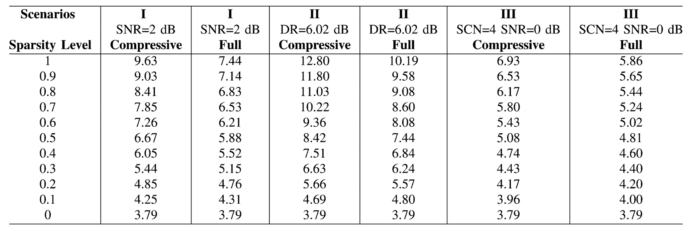
\includegraphics[width=0.75\columnwidth]{figs/csp-soe.png}
\DeclareGraphicsExtensions.
\caption{Block diagram of lookup table for sparsity order estimation through signal-to-noise ratio (SNR) and asymptotic eigenvalue probability distribution function (aepdf). For example, if the value of aepdf = 7.26 for the compressive case in SNR = 2db, it can be estimated that the sparsity order of spectrum occupancy is 0.6}\label{csp-soe}
\end{figure}

\subsubsection{Noise Level Estimation}

For CR networks, the signal-to-noise ratio (SNR) affects the performance of spectrum detectors. For example, the energy detector (ED) is simple and fast, but with poor performance in low SNR scenarios; Feature detectors (FD) are complex and slow, but have strong robustness to noise. In \cite{sharma2014compressive_snr}, the author similarily build up a lookup table relating the noise estimation with the eigenvalue probability distribution function in covariance matrix of the compressively sampled primary signal. 

Then if we have the access to estimate the SNR in CRN, we can achieve the following spectrum sensing approach in the future: 

\paragraph{Hybrid Spectrum Sensing} 

If we have known the SNR, we can design a more intelligent two stage detector. In the coarse stage, a quick search is done over a wide bandwidth, and in the fine stage, the sensing is done over the individual candidate sub-bands in that bandwidth, one at a time. the coarse stage is based on energy detection due to its fast processing. If the test statistics is larger than a predefined threshold, then the band is considered occupied. Otherwise, a fine stage is performed where a cycle-stationary detector is implemented due to its robustness at the low SNR regime. (For sparsity level, we can judge whether the CS based detector suitable if there exists dense channel occupancy by primary users)

\paragraph{Adaptive spectrum Sensing} 

In case when a CR successfully know the primary signals' SNR, the CR can intelligently choose optimal detection algorithms based on SNR related performance of detectors. For instance, if the SNR is detected to be very low, then cycle-stationary detection algorithm can be used due to its robustness at the low SNR regime. Otherwise, the energy detector can be used since it's fast and accurate enough in high SNR regime. Extending this idea of selecting various of detector based on CSP estimation, we can select the optimal detector adaptively. This will provide future cognitive radio more flexibility to the varying environment.

\subsection{Other Related Wideband Processing with CSP}

\subsubsection{CSP based TOA for UWB Positioning}\label{sct:csp_toa}

Maximizing the cross-correlation between the two signals is one of the key steps in time-of-arrival (TOA) algorithms which have been applied in compressive UWB positioning in chapter \ref{C:compressive_uwb_positioning}. In that system, the procedures at receiving end can be abstracted as (1) low-rate sampling, then (2) CS fully reconstruction, finally (3) TOA algorithm based locationing. However, the (2) CS fully reconstruction may sometimes Not necessary if we borrow the theorem.

According to \cite{ohlsson2013compressive}, where the shift retrieval problem for compressive samples is investigated, we may directly recognising the shift distance from CS data without recovery. Now the thoerem has not been embedded into UWB positioning, so the CSP-TOA positioning is a possible research application in the future.

\begin{figure}[!t]
\centering
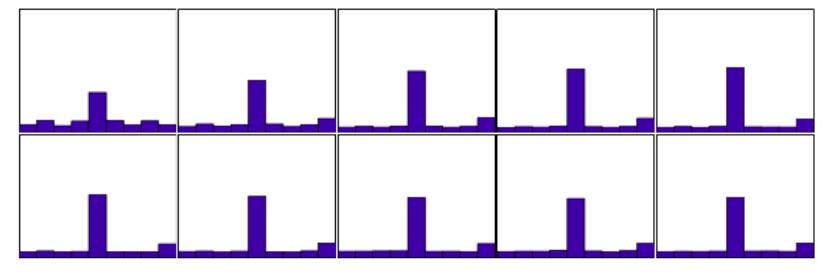
\includegraphics[width=0.75\columnwidth]{figs/csp-shift.png}
\DeclareGraphicsExtensions.
\caption{Histogram for the estimated shift in SNR = 2. From left to right, top to bottom, compression ratio = 0.1 ... 1. The true shift was set to 5 in all trials}\label{csp-shift}
\end{figure}

\subsubsection{CSP based Demodulation}

A compressive sensing phase-locked loop (CS-PLL) \cite{schnelle2012compressive}, is designed for directly extracting the phase and frequency from compressively sampled modulated signal $without$ sparse recovery. Since the restricted isometry property (RIP) of CS ensures that the standard inner product between $x[n]$ and $u[n]$ is approximately the same as that in the compressively sensed version produced by $y[m]$ and $u[n]$ \cite{davenport2010signal}, hence, the inner products in the standard PLL and that in the CS-PLL are nearly the same, ensuring the consistence between the standard PLL $\theta [n]$ and the CS-PLL's output $\theta [m]$. The presentation of the $\theta [m]$ can be presented as $\theta [m] = \sum_{k} y[k]v[k]h[m-k]$, where the index $m$ indicates the lower sampling rate compared with the Nyquist rate index $n$. In addition, the compressive sensing operations $\Phi$ which apply the RD's architecture consist of a input pseudo-random sequence, a mixer, a integrator, and a low-rate sampling ADC, which is the same as the random demodulator's architecture in chapter 2.

This CS-PLL has many application fields if the FM demodulation is necessary in compressive sensed data. When we successfully apply this technique, we don not need recovery, but directly demodulate original information from the received modulated signals.

\begin{figure}[!t]
\centering
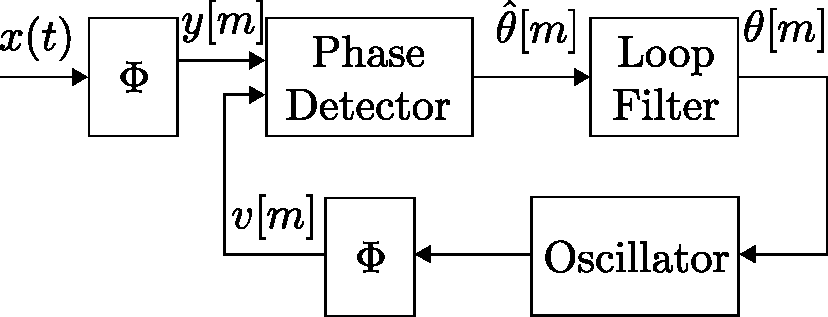
\includegraphics[width=0.5\columnwidth]{figs/pll2.pdf}
\DeclareGraphicsExtensions.
\caption{Block diagram of the compressive sensing phase-locked loop (CS-PLL). The components includes the pre-CS sampler, phase detector, loop filter, oscillator and the feed-back CS multiplier}\label{CS-PLL}
\end{figure}

\section{Conclusion}

In the this chapter, we have followed the discussion of the main drawback in compressed sensing based spectrum sensing (CS-CSS) which derives from the computational non-linear CS reconstruction, and then propose the idea of signal processing directly on compressively sampled data (CSP) without fully recovery. Then we introduce our future potential work which will embed CSP into cognitive spectrum sensing, including CSP based filtering, CSP based detection, and CSP based estimation. Some other possible CSP applications in UWB positioning and signal demodulation are also introduced. We hope that by utilise the CSP in spectrum sensing, a high real-time performance, high flexible ,energy efficient hardware could be achieved in the future. 

%--------------------------------------------------------------

%As a fact, the CS framework sacrifices the time and energy performance in reconstruction produce (in return, the sampling rate is reduced). In order to solve this problem, this chapter focuses on exploring the potential approach of directly analysing compressive measurements without fully CS reconstruction. The new approach is termed as compressive signal processing (CSP), and it will be used for compressive spectrum sensing (CSS) in cognitive radio (CR), so that the drawback will be overcome. 

%In conclusion, the motivations for developing signal processing for compressed measurements can be categorised in following aspects:

%\paragraph{Demand for simple signal processing in CS}
%The reconstruction algorithms for CS is non-linear, which indicates that the recovered data are not directly suitable for conventional digital signal processing where a simple recovery using cardinal sine (sinc) interpolation (linear process) is required. One solution is to sequentially achieve CS reconstruction and then process the recovered data, but it's too computational expensive.

%\paragraph{Requirement for energy efficiency in CS}

%The discussion in chapter \ref{C:wideband_css} stresses the main drawback in CS based cognitive spectrum sensing. which derives from the computational non-linear CS reconstruction.


% %--------------------------------------------------------------
% 
% \section{Interference Avoidance}
% 
% Assume a sparse signal $x \in R^N$ which consists of two components:
% \begin{equation}
% \label{csp1}
% x = x_s + x_I, \quad x_S \in S_S\; and\; x_I \in S_I
% \end{equation}
% , where the $x_S$ contains the spectrum of interest and the $x_I$ stands for the useless information. After the CS acquisition, we gain $y = \Phi x = \Phi(x_S + x_I)$. Then our aim is to wipe out the contribution of $\Phi x_I$ from the observation $y$ before recovering $x$. The following theorem provide the applicability of this idea:  
% \begin{theorem}\cite{davenport2010signal}
% \label{csp2}
% Suppose that $\Phi$ satisfies the $\delta$-stable RIP for all $x_S\in\Sigma_S$ and $x_I\in\Sigma_I$, where $I$ is a $K_I$ dimensional subspace of $R^{N}$. Assume that $\Psi_I$ is an matrix whose columns constructs an orthogonal basis for the $K_I$ dimensional subspace. Define the matrix $P_{\Omega} = \Phi\Psi_I(\Phi\Psi_I)^{\dagger}$ and $P_{\Omega^{\perp}} = I-P_{\Omega}$. For any $x \in \Sigma_S \cup \Sigma_I$, we regard $x = x_S + x_I$, where $x_S \in s_S$ and $x_I \in s_I$, then
% \begin{equation}
% \label{csp3}
% P_{\Omega^{\perp}} \Phi x = P_{\Omega^{\perp}} \Phi \hat x ,\quad
% \frac{\delta}{1-\delta} \leq \|P_{\Omega^{\perp}} \Phi \hat x\|_2 \leq 1 + \delta 
% \end{equation}
% \end{theorem}
% The theorem \ref{csp2} proofs that there exists a matrix $P_{\Omega^{\perp}}$ which is nearly orthogonal to the useless information $x_I$ such that $P_{\Omega^{\perp}} x_I \approx 0$. Hence the matrix $P_{\Omega^{\perp}}$ is the filter for selecting the desired signal $x_S$. we can apply this theory to construct a $filtering matrix$ in CS acquisition model if the support of the $x_I$ is known. 
% In addition, it also points out that $P_{\Omega^{\perp}}\Psi$ satisfies the $\delta/(1-\delta)$-stable RIP for all $x \in \Sigma_{S_S}$, indicating that this filtering matrix provide a stable recovery:  
% \begin{theorem}\cite{davenport2010signal}
% \label{csp4}
% Suppose that $\Phi$ satisfies the $\delta$-stable RIP for all $x_S\in\Sigma_S$ and $x_I\in\Sigma_I$, where $I$ is a $K_I$ dimensional subspace of $R^{N}$. Assume that $\Psi_I$ is an matrix whose columns constructs an orthogonal basis for the $K_I$ dimensional subspace. Define the matrix $P_{\Omega}$ and $P_{\Omega^{\perp}}$ as in the theorem \ref{csp2}. Then the $P_{\Omega^{\perp}}\Phi$ satisfies $\delta/(1-\delta)$-stable RIP for all $x_S \in \Sigma_S$ and $P_{\Omega}\Phi$ satisfies $\delta$-stable RIP for all $x_I \in \Sigma_I$.  
% \end{theorem}
% 
% 
% 
% \paragraph{Requirement for real time ability in CS}
% \section{Compressive Estimation}
% \subsection{Compressive Phase-Locked Loop}
% Since computationally expensive for accurate sparse recovery is relatively high which reduces the real-time processing ability of CS devices, a compressive sensing phase-locked loop (CS-PLL)  \cite{schnelle2012compressive}, is designed for directly extracting the phase and frequency from compressively sampled modulated signal $without$ sparse recovery. This novel architecture brings computational advantages that improves the real-time processing capability in CS devices such as FM receivers\cite{davenport2010wideband} and widely implemented in wireless communication. 
% 
% %It applies a revised PLL structure by adding two compressive sensing (CS) operations $\Phi$ to the original standard architecture of PLLs: one operation is the pre-CS sampler representing the random demodulator (RD) for modulated signal acquisition; another one is the feed-back multiplier which has the same structure as the first, which locates between the oscillator and the phase detector. Then the new architecture of the CS-PLL is shown in Figure \ref{CS-PLL}, comprised of a pre-CS sampler, phase detector, loop filter, oscillator and a feed-back CS multiplier.
% 
% \begin{figure}[!t]
% \centering
% 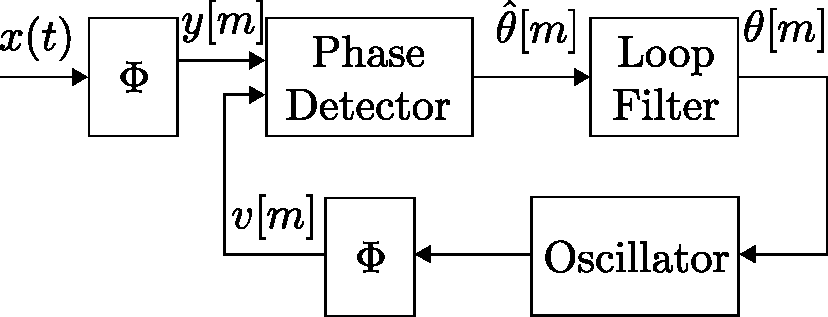
\includegraphics[width=2.2in]{figs/pll2.pdf}
% \DeclareGraphicsExtensions.
% \caption{Block diagram of the compressive sensing phase-locked loop (CS-PLL). The components includes the pre-CS sampler, phase detector, loop filter, oscillator and the feed-back CS multiplier}\label{CS-PLL}
% \end{figure}
% 
% Since the restricted isometry property (RIP) of CS ensures that the standard inner product between $x[n]$ and $u[n]$ is approximately the same as that in the compressively sensed version produced by $y[m]$ and $u[n]$\cite{davenport2010signal}, hence, the inner products in the standard PLL (\ref{eqn_pll1}) and that in the CS-PLL (\ref{eqn_pll2}) are nearly the same, ensuring the consistence between the standard PLL $\theta [n]$ and the CS-PLL's output $\theta [m]$. The presentation of the $\theta [m]$ can be presented as:
% \begin{equation}
% \label{eqn_pll2}
% \theta [m] = \sum_{k} y[k]v[k]h[m-k]
% \end{equation} 
% , where the index $m$ indicates the lower sampling rate compared with the Nyquist rate index $n$. In addition, the compressive sensing operations $\Phi$ which apply the RD's architecture consist of a input pseudo-random sequence, a mixer, a integrator, and a low-rate sampling ADC, which is the same as the RD's architecture shown in Figure \ref{RD}.
% 
%--------------------------------------------------------------

%\section{Compressive Sensing Processing} 

%\subsection{Applications: CSP Detector}

%the CSP-detector which estimates the existence of primary users directly from CS samples before recovery, so running time is significantly saved. Further, CS-filters, CS-estimators etc can also embedded for other scenarios in cognitive spectrum sensing, in order to improve the real-time capability direction, or further adaptive sensing schemes. Also, our future research direction will follow this idea.

%In this section, compressed sensing based spectrum sensing techniques for cognitive radio are introduced and compared. As a result, traditional sensing techniques of CR such as energy detector, feature detector can improve their detection performance if they implement the CS technique under the assumption that sensed spectrum are sparse. However, as the CS reconstruction requires non-linear processing which is much complex than traditional linear sinc based recovery, the real-time capability loss becomes the main payment for reducing the high sampling rate problem aforementioned in this chapter. Besides, the CS techniques highly relies on the assumption that object (spectrum) are sparse, in other words, CS is not  suitable for dense wireless communication environment. These two problems lead the following discussion in the next chapter, which shows our proposed research directions. 

%\section{Compressed Signal Processing for Cognitive Radio}\label{C:csp_cr}

%In aforementioned sections, compressed sensing based spectrum sensing techniques for cognitive radio are introduced and compared. As a result, traditional sensing techniques of CR such as energy detector (ED), coherent detector (CD) can improve their detection performance if they implement the CS technique under the assumption that sensed spectrum are sparse. However, as the CS reconstruction requires non-linear processing which is much complex than traditional linear sinc based recovery [xx-yy], the real-time capability loss becomes the main payment for reducing the high sampling rate problem aforementioned in this chapter. Besides, the CS techniques highly relies on the assumption that object (spectrum) are sparse, in other words, CS is not  suitable for dense wireless communication environment. These two problems lead the following discussion in the next chapter, which shows our proposed research directions. 

%In this chapter, we propose a potential approach, term as the compressive signal processing (CSP) [x], to enhance the real-time capability of compressed sensing based cognitive sensing framework under the assumption that in many cases fully recovery is NOT necessary. Followed by this idea, [xx-yy] successfully reduce the executive time since the magnitude of recovered signal length is significantly decreased. On the other hand, since cognitive spectrum sensing (CSS) only requires detecting the 'existence' of spectrum, so fine recovery is no need. From this aspect, the idea of CSP is well suited for CSS. In this chapter, an overview of the compressed signal processing (CSP) theory is presented, as well as the CSP-based applications in wireless communications. 

%In this chapter, we propose an overview of cognitive radio (CR) networks and then focus on the bottleneck in its front-end sampling devices. Due to the wideband sensing task in CR, the required sampling rate becomes extremely high. Although various approaches [xx-yy] are recently developed to solve this problem, it's shown that in many scenarios, the compressed sensing is the optimal method to solve the problem [xx-yy]. This chapter presents the recent work of compressed spectrum sensing for cognitive radio.

%-------------------------------------------------------------------------------------------------------------

%\section{Motivation}\label{sct:csp_moti}

%In the last chapter, compressed sensing based spectrum sensing techniques for cognitive radio are puzzled by the heavy burden from non-linear CS reconstruction procedure [xx-yy]. Previous approaches such as greedy recovery [xx-yy] aims at fast reconstruction while keeping considerable robustness, and they achieve to present enough contributions. 

%Besides, the CS techniques highly relies on the assumption that object (spectrum) are sparse, in other words, CS is not  suitable for dense wireless communication environment. These two problems lead the following discussion in the next chapter, which shows our proposed research directions. 

%--------------------------------------------------------------

%Besides, since accurate detection of cognitive spectrum sensing is always required for not interfering primary users, time consuming algorithms -- convex optimization (e.g.basis pursuit) is needed. In such cases, large delays are generated and in conflict with agility (i.e. feedback reconfiguration) in cognitive radios. 

%--------------------------------------------------------------

%However, in CS acquisition model, this relation no longer remains indicating we cannot directly achieve CS based signal processing without recovering the original data. What's worse, CS based reconstruction is always complicated than that in traditional Nyquist theory based ADCs: In traditional ADCs, signal reconstruction can be achieved by $sinc$ interpolation which is a linear processing with little computation, while the CS based signal reconstruction requires nonlinear computations such as convex optimization based or greedy pursuit algorithms, which are considered as  more computationally expensive\cite{davenport2010signal}. Therefore, the signal processing becomes a crucial problem in acquisition systems using CS based ADCs. 

%--------------------------------------------------------------

%Signal processing through compressive measurements is always difficult than that by traditional one. In traditional Nyquist theory framework, the signal processing applies the relation between the spectrum and time domain samples, which makes the digital processing operations easily replaced by their continuous counterparts \cite{mishali2011xamplingsignal}. Digital filtering exploits this relation, as well as estimation, detection and classification.
%}

%---------------------------------------------------------------

%\section{Conclusion}
%In the last chapter \ref{C:wideband_css}, we have discussed that the main drawback of compressed sensing based spectrum sensing (CS-CSS) lies in the non-linear CS reconstruction. As a fact, the CS enhance the performance in sampling but sacrifice the one in reconstruction produce -- the computational complexity for CS reconstruction brings heavy cost in both time cost and energy cost. 

%---------------------------------------------------------------

%\paragraph{Real-Time Capability}
%The reconstruction algorithms for CS is non-linear, which indicates that the recovered data are not directly suitable for conventional digital signal processing where a simple recovery using cardinal sine (sinc) interpolation (linear process) is needed. Besides, since accurate detection of cognitive spectrum sensing is always required for not interfering primary users, time consuming algorithms -- convex optimization (e.g.basis pursuit) is needed. In such cases, large delays are generated and in conflict with agility (i.e. feedback reconfiguration) in cognitive radios. 

%\paragraph{Energy Efficiency}
%The heavy reconstruction for CS not only brings large time-delay, but also additional energy cost. Compared to linear recovery in traditional approaches, the CS based signal detection additionally required the block for spectrum recovery before further hypothesis detection. Then here comes the question: what if we directly perform hypothesis detection without CS reconstruction ? If the idea is achievable, the additional energy cost will be eliminated so that the entire energy reduces. Besides, not only detection, if we can expand this idea to filtering, estimation, then more intelligent-based scheme for cognitive radio can be supported in physical layer. 


%To our best knowledge, most of CSP based cognitive spectrum sensing do Not involves energy aware design. 

%Our aims for following the CSP are (1) find energy-efficient solution for cognitive spectrum sensing, and (2) solve the real-time capacity to enhance the overall performance of compressive CRs. Since the CSP applications are still relying on various conditions, such SNR, Taps of filters, length of original signal, 

%\section{CSP Theory for Cognitive Spectrum Sensing}\label{sct:csp_theory}
%In many scenarios, the aim of CS fully recovery is no longer necessary, and directly analysis or partial recovery then analysis become possible and applicable. This section briefly presents CSP theory by various topics relating to our research area of cognitive radio spectrum sensing. Theories for CSP based filtering, estimation, interference avoidance, classification, shift retrieval, sparsity order prediction are briefly introduced.

%--------------------------------------------------------------

%Further, Guo et al develops CSP for feature detector in \cite{guo2013feature} and pattern clustering is achieved.

%--------------------------------------------------------------

%In some noise cases, only parts of certain information from measurements are needed, and thus we prefer to filter out the useless information before further signal processing. Therefore, if we could estimate the useless information corresponding to some observations, and then $throw$ them $away$ before CS based signal recovery, we can avoid a high computational complexity and thus save the power efficiency significantly. According to \cite{Theorem 1, davenport2010signal}. 

%\chapter{Conclusion}\label{C:conclusion}

\indent \indent To the best of our knowledge, the aforementioned compressed signal processing (CSP) technique has not been fully developed, because as the interest of signal changes in different environment, spectrum that does Not need "fully recovery" (e.g. interfere and unrelated frequency bands) also varies. In other words, many potential spectrum sensing application based on CSP are still worth developing under different cases. 

In this chapter, our future work is introduced. The work follows the recent research of the CSP, implemented on cognitive spectrum sensing (CSS), and focus on how to directly get enough informations from partial compressed measurements, or without any recovery. This topic involve innovative filtering and estimation method for compressed signals (as research goes on, maybe classification will also be involved. Our final aim is to embed these technique to reduce the hardware complexity and improving its real-time capability for cognitive radio devices. 

%-------------------------------------------------------------------------------------------------------------
\section{Contributions}\label{sct:Contribution}
\indent \indent In our research of AMS tracking algorithm, there are three major contributions in the following aspects:

\paragraph{Image Representation:} We design an adaptive fusion mechanism of IPCA (Incremental Principle Component Analysis) and color histogram. The IPCA represent the object as an incrementally updated eigenspace, where IPCA is robust to adapt the multi-view of the object and distortions leading by illumination variations and rotations. However, as the IPCA method uses the wrapped image patch of the object, it is very sensitive against the shape deformation of pliable objects. The color histogram feature is used as a complementary feature to the IPCA in our method, where color histogram discards the spatial information. We adaptively adjust the weights of the representation method in our reference appearance model, based on the discrimination of the color histogram feature between the object and the background.

\paragraph{Appearance Model:} To avoid the error accumulation in appearance model updating, we propose our AMS tracking method. We copy the object appearance information into a new initialized appearance model before big transformations in video sequence (\emph{e.g.}, occlusion, appearance variation, fast movement and cluttered background). If the transformation is allowed like appearance variation and fast movement, the updated reference model during the transformation would be selected in the following tracking. But if it is invalid transformation like collusion and cluttered background, the new initialized model is selected after the transformation. This mechanism is able to avoid error accumulation in model updating successfully.

\paragraph{Implementation:} We implement the AMS tracking algorithm with MATLAB and do the comparison with some recently popular visual tracking algorithms. The accuracy and analysis are given. We also test the computation efficiency of our AMS tracking algorithm against iVT \cite{iVT2008} tracking.

%-------------------------------------------------------------------------------------------------------------
\section{Recommendations for Future Work}\label{sct:FutureWork}
\indent \indent The following are three directions of our future work in surveillance system.

\subsection{Time Efficient Algorithms}
\indent \indent The accuracy of our proposed AMS tracking algorithm is good compare to the recently popular visual tracking algorithms. However, the time overhead of the proposed algorithm is more than iVT algorithm, where only iVT is also implemented with MATLAB in the compared algorithms. The additional computation complexity comparing to iVT algorithm is in the appearance selection mechanism, as each model in the model pool requires the computing of the related reliable function. In the proposed method, the reliable function in each frame is independent, and we need to do the same computing in each frame. One way of reducing the time overhead is to incrementally update the reliable functions frame by frame. The computational complexity reducing problem is an important issue in future research of object tracking.

\subsection{Multimodal Surveillance}
\indent \indent Another direction of our future work is multimodal surveillance, where multimodal sensors are integrated into the system including video, audio, IR radiation, laser, vibration and some biometric sensors. The multimodal surveillance system has the capability to work in complex and rugged environments (\emph{e.g.}, night and dust background), detect dissembling targets and provide more feature details of the targets with biometric sensors. The challenges in multimodal surveillance system mainly include: multiple sensor control techniques and multimodal integration algorithms.

\paragraph{Multiple Sensor Control Techniques:} mainly focus on the problem of most efficiently exploring the capability of each sensor and broadening the territory of the surveillance area with limited sensors. It asks the cameras to be calibrated with specifical parameters by considering the location, viewpoints of the related camera. The configuration of all the sensors installation is another important issue. The overlapping area of different sensors should be considered in order to find the related objects while maximizing the surveillance area at the same time.

\paragraph{Multimodal integration algorithms} is to effectively integrate the data from different multimodal sensors. The different data types can lead to the improvement of the detection and tracking accuracy. The problem in multimodal integration includes synchronization of sensors, corresponding objects finding in multiple sensors, and data transmission methods. In our future work, we will focus on some common sensors integration like video, audio and infrared.

\subsection{Object Behavior Analysis}
\indent \indent Object behavior analysis is another challenging issue in surveillance system. It is an important part of event detection and relies on the output of the object detection and tracking algorithm. The behaviour analysis problem can be formulated as a classification problem by matching the detected time varying features to the pre-defined image sequence. However, due to the complexity of the interactions and activities that have flexible representations, behavior analysis problem can be addressed by using rule-based inference, causal analysis, physical constraints and syntactic analysis.

Our future work on this area will focus on efficiently using the data results from the object detection and tracking step and improve the detection and tracking by feeding back the object behavior. Like when we analyze crowd behaviours, we can model the targets as bounding box or points in object detection and tracking. But in the situation of understanding the behaviour of a suspicious person, it is better for us to model the body with articulated model to get the trajectories of each part of the body. Besides, the object behavior analysis result can give feedbacks to the detection and tracking by estimating the possible states of the object in the incoming frames.
%-------------------------------------------------------------------------------------------------------------
\section{Submitted Papers}

\begin{enumerate}[{[}1{]}]
  \item Y. Yuan, S. Emmanuel and W. Lin, “Appearance Model Selection in Visual Object Tracking,” International Conference on Acoustics, Speech, and Signal Processing (ICASSP 2013), Submitted,  Vancouver, Canada, May 2013.
  \item Y. Yuan, S. Emmanuel and W. Lin, “Robust Visual Tracking via Appearance Model Selection,” IEEE Transaction on Multimedia, Submitted.
\end{enumerate}


\bibliographystyle{IEEEtran}
\bibliography{Reference}

\end{document}
